%% 
%% Copyright 2007-2020 Elsevier Ltd
%% 
%% This file is part of the 'Elsarticle Bundle'.
%% ---------------------------------------------
%% 
%% It may be distributed under the conditions of the LaTeX Project Public
%% License, either version 1.2 of this license or (at your option) any
%% later version.  The latest version of this license is in
%%    http://www.latex-project.org/lppl.txt
%% and version 1.2 or later is part of all distributions of LaTeX
%% version 1999/12/01 or later.
%% 
%% The list of all files belonging to the 'Elsarticle Bundle' is
%% given in the file `manifest.txt'.
%% 

%% Template article for Elsevier's document class `elsarticle'
%% with numbered style bibliographic references
%% SP 2008/03/01
%%
%% 
%%
%% $Id: elsarticle-template-num.tex 190 2020-11-23 11:12:32Z rishi $
%%
%%
\documentclass[preprint,12pt]{elsarticle}

%% Use the option review to obtain double line spacing
%% \documentclass[preprint,review,12pt]{elsarticle}

%% Use the options 1p,twocolumn; 3p; 3p,twocolumn; 5p; or 5p,twocolumn
%% for a journal layout:
%% \documentclass[final,1p,times]{elsarticle}
%% \documentclass[final,1p,times,twocolumn]{elsarticle}
%% \documentclass[final,3p,times]{elsarticle}
%% \documentclass[final,3p,times,twocolumn]{elsarticle}
%% \documentclass[final,5p,times]{elsarticle}
%% \documentclass[final,5p,times,twocolumn]{elsarticle}

%% For including figures, graphicx.sty has been loaded in
%% elsarticle.cls. If you prefer to use the old commands
%% please give \usepackage{epsfig}

%% The amssymb package provides various useful mathematical symbols
\usepackage{amssymb}
%% The amsthm package provides extended theorem environments
%%\usepackage{amsthm}

%% The lineno packages adds line numbers. Start line numbering with
%% \begin{linenumbers}, end it with \end{linenumbers}. Or switch it on
%% for the whole article with \linenumbers.
\usepackage{lineno}

%% Русский язык - закомментировать в финальной версии
%\usepackage[russian]{babel}

%% advanced mathematics
\usepackage{amsmath}
\usepackage[ruled]{algorithm2e}
\usepackage{multirow}

\usepackage{graphicx}
\usepackage[table,xcdraw]{xcolor}
\usepackage{amssymb}

\usepackage{hyperref}

\journal{Knowledge-Based Systems}

\begin{document}

\begin{frontmatter}

%% Title, authors and addresses

%% use the tnoteref command within \title for footnotes;
%% use the tnotetext command for theassociated footnote;
%% use the fnref command within \author or \address for footnotes;
%% use the fntext command for theassociated footnote;
%% use the corref command within \author for corresponding author footnotes;
%% use the cortext command for theassociated footnote;
%% use the ead command for the email address,
%% and the form \ead[url] for the home page:
%% \title{Title\tnoteref{label1}}
%% \tnotetext[label1]{}
%% \author{Name\corref{cor1}\fnref{label2}}
%% \ead{email address}
%% \ead[url]{home page}
%% \fntext[label2]{}
%% \cortext[cor1]{}
%% \affiliation{organization={},
%%             addressline={},
%%             city={},
%%             postcode={},
%%             state={},
%%             country={}}
%% \fntext[label3]{}

\title{On hyperparameter tuning through Lipschitz global optimization} % and dimensionality reduction}?
%% О настройке гиперпараметров с помощью липшицевой глобальной оптимизации

%% use optional labels to link authors explicitly to addresses:
%% \author[label1,label2]{}
%% \affiliation[label1]{organization={},
%%             addressline={},
%%             city={},
%%             postcode={},
%%             state={},
%%             country={}}
%%
%% \affiliation[label2]{organization={},
%%             addressline={},
%%             city={},
%%             postcode={},
%%             state={},
%%             country={}}

\author[UNN,ITMO]{Konstantin Barkalov\corref{cor}}
\cortext[cor]{Corresponding author: \url{konstantin.barkalov@itmm.unn.ru}}
\author[UNN,ITMO]{Denis Karchkov}
\author[UNN,ITMO]{Evgeny Kozinov}
\author[UNN,ITMO]{Ilya Lebedev}
\author[UNN,ITMO]{Denis Rodionov}
\author[UNN,ITMO]{Marina Usova}

\affiliation[UNN]{organization={Lobachevsky University},%Department and Organization
            addressline={Gagarin Av. 23}, 
            city={Nizhni Novgorod},
            postcode={603022}, 
            %state={},
            country={Russia}}
						
\affiliation[ITMO]{organization={ITMO University},%Department and Organization
            addressline={Lomonosova St. 9}, 
            city={St. Petersburg},
            postcode={191002}, 
            %state={},
            country={Russia}}



\begin{abstract}
%% Text of abstract

The quality of machine learning methods is substantially affected by their hyperparameters, while the evaluation of the quality criterion is a time-consuming operation. Therefore, it is important to develop intelligent methods for selecting optimal values of hyperparameters that require a small number of search trials. In this paper, we propose a new approach to hyperparameter tuning based on the ideas of Lipschitz global optimization. In the framework of this approach, the solution of problems with several parameters is reduced to solving equivalent one-dimensional problems. The reduction is based on the use of space-filling curves (Peano curves). These approaches are implemented in the iOpt open-source framework of intelligent optimization methods.  To demonstrate the advantages of iOpt, we compare it with the well-known Optuna and HyperOpt frameworks when tuning hyperparameters of various machine learning methods on a representative set of datasets. The results show that Lipschitz global optimization methods provide comparable (in terms of quality) results in a significantly shorter time compared to known hyperparameter tuning algorithms.

\end{abstract}

%%Graphical abstract
%\begin{graphicalabstract}
%\includegraphics{grabs}
%\end{graphicalabstract}

%%Research highlights
\begin{highlights}
\item A framework of Lipschitz optimization methods is developed for the tuning of hyperparameters
\item Dimensionality reduction based on Peano space-filling curves is used to solve multidimensional problems
\item A scheme is proposed for reducing the problems, some of whose parameters are categorical, to a single problem with continuous parameters
\item The developed methods (unlike the known methods of hyperparameter tuning) are deterministic, which ensures stable results at different runs of the algorithms 

\end{highlights}

\begin{keyword}
%% keywords here, in the form: keyword \sep keyword
Lipschitz optimization \sep Global optimization \sep Multiextremal functions \sep Hyperparameter tuning

%% PACS codes here, in the form: \PACS code \sep code

%% MSC codes here, in the form: \MSC code \sep code
%% or \MSC[2008] code \sep code (2000 is the default)

\end{keyword}

\end{frontmatter}

\linenumbers

%% main text
\section{Introduction}
\label{sec_intro}

Currently, complex scientific and/or industrial problems are most often solved by numerical methods. Most of such methods, for example, machine learning methods, have hyperparameters, and the choice of specific values of these hyperparameters can determine the efficiency (in a given metric) of the obtained solution under certain constraints on the computation time \cite{Hutter2019,nikitin2021}. The fact that in many cases the difference in the efficiency of the solution obtained with different values of hyperparameters can be quite significant, has resulted in the emergence of the hyperparameter optimization (HPO) problem, as well as the research of approaches to its solution that are implemented in the frameworks for automatic selection of hyperparameters \cite{Tune, optuna, hyperopt,Sherpa}. From the mathematical point of view, the HPO problem corresponds to a global optimization problem with fixed bounds on the variation of hyperparameters.  In certain cases, some of the hyperparameters may be categorical, i.e., they can only assume values from a certain, usually small, number of variants, which necessitates the use of optimization methods capable of solving problems with discrete parameters.

For an end user who wishes to fine-tune the method used by selecting an optimal combination of hyperparameters, the choice of a particular framework is determined by the following factors: 1) efficiency of the methods implemented in the framework that allow solving an HPO problem from the class of problems to which the user's problem belongs; 2) ease of using the  framework from the point of view of description/formulation of the problem of selecting the optimal combination of hyperparameters, organization of the optimum search process, as well as obtaining and analyzing the results. Today, the most common way to organize such an interface is to use the Python programming language, while the frameworks can be written both in this and other languages.

In this paper, we present iOpt\footnote{\url{https://github.com/aimclub/iOpt/}}, a framework of intelligent optimization methods focused on solving problems of selecting optimal values of hyperparameters of various algorithms (including machine learning and heuristic optimization methods). The paper is organized as follows. At the beginning, there is a review of known methods used for hyperparameter tuning. Section \ref{sec_lip} presents the mathematical formulation of the problem, describes approaches to the reduction of multidimensional problems to one-dimensional problems and to the solution of problems with discrete parameters. Section \ref{sec_iOpt} explains the algorithmic basis of global optimization methods implemented in the iOpt framework. In Section \ref{sec_exp}, we present the results of numerical experiments conducted to compare the efficiency of the iOpt framework with other known frameworks on model and applied problems. The conclusion summarizes the findings and plans   for the development of the framework.


\section{Related work}
\label{sec_rel}

The main difficulty in solving the HPO problem is that the search for the optimal combination of hyperparameters requires for each selected variant of their values to solve the corresponding initial problem, for example, the problem of machine learning, and thus can take quite a long time. Thus, any approach to solving the HPO problem will be limited by the number of combinations of hyperparameters that the global optimization method can test before the available computational resource is exhausted.  Certainly, it is difficult in such circumstances to speak about convergence of the method to the global optimum or about any guarantees of finding it. We can only consider the possibility of obtaining an acceptable (from the researcher's point of view) solution. Let us briefly characterize a number of methods that are used to tune hyperparameters (depending on the properties of the initial problem). 

The simplest way to find the global optimum is the exhaustive search method (search on a uniform \cite{Bao2006} or random \cite{Bergstra2012} grid). 
By selecting the number of analyzed variants for each of the hyperparameters, searching all the resulting combinations and choosing the best of them in a given metric, we obtain an estimate of the optimum with a certain accuracy \cite{Nevendra2022}. The exhaustive search method is easy to implement, it has perfect parallelism, but it has a significant drawback (an exponential growth of the number of grid nodes as the number of hyperparameters increases). Thus, exhaustive search can be used as a method for solving HPO problems only in ``simple'' problems where both the number of hyperparameters (one or two) and the time for solving the initial problem with each selected combination of hyperparameters are small. 

Metaheuristic (genetic and similar) algorithms are an alternative to the exhaustive search when the number of hyperparameters increases \cite{Opara2019}. These algorithms are widely used in the absence of a formula-based description of the model under study (``black-box'' model), which is typical for the considered HPO problems \cite{Zhou2021,Yang2022}. Metaheuristic algorithms only weakly depend on the number of hyperparameters, they use information from previous iterations to perform the current one, but due to the randomness inherent in the methods, they guarantee the finding of the global optimum only in the probabilistic sense.

Another approach to finding the global optimum is Bayesian optimization, which is also used to solve ``black-box'' problems \cite{Frazier2018,Archetti2019}. In fact, Bayesian optimization methods build a stochastic model of the function being optimized. The model is iteratively updated on the basis of the information accumulated in the process of searching for the optimum, making it possible to estimate the most probable position of the global optimum at each iteration. Bayesian optimization methods have significantly higher efficiency compared to the exhaustive search, but they are also affected by the ``curse of dimensionality'', albeit to a lesser extent. 

In well-known hyperparameter tuning frameworks, the Tree-Structured Parzen Estimator (TPE) algorithm is widely used \cite{hyperopt,NIPS2011}. TPE is an iterative algorithm, conceptually close to Bayesian optimization methods. Before the algorithm starts, a search region in the hyperparameter space must be specified and the function to be optimized must be defined. In the course of its work, the method performs trials in the search region and then uses these trials to construct estimates of the distribution of the best and all other results in the hyperparameter space. Next, the combination of hyperparameters that gives the maximum expected improvement is searched for. These hyperparameters are then evaluated on the objective function. The described process is repeated until a specified number of iterations is attained or until the time constraint is reached.  

The good results achieved by Bayesian optimization \cite{Joy2020} and TPE \cite{Watanabe2022a,Watanabe2022b} methods are based on the a priori assumption that the function corresponds to a certain stochastic model, such as a Gaussian process \cite{Rasmussen2005}. However, there are other assumptions about the shape of the function in global optimization that yield remarkable results. 

One of such assumptions about the problem to be solved is the assumption of boundedness of relative changes in the objective function. In this case, the function is said to satisfy the Lipschitz condition, and the problem to be solved is called a Lipschitz global optimization problem. For the class of Lipschitz global optimization problems, a number of efficient algorithms have been developed \cite{Jones2021,Paulavicius2020,Strongin2020,Sergeyev2017,PaulaviciusZilinskas2014}, which surpass many other global optimization methods \cite{Sergeyev2018} and have shown their applicability in a number of applications \cite{Kvasov2008,CANDELIERI2019,Gubaydullin2021}.

The iOpt framework contains an implementation of Lipschitz optimization algorithms, which are an extension of the information-statistical global search algorithm described in detail in \cite{Strongin2000,Sergeyev2013}. In particular, the methods have been adapted to solve problems with partially integer parameters, which are very common in HPO problems. The experimental results presented in Section \ref{sec_exp} show that the iOpt framework is not inferior in HPO problems to well-known frameworks having the same purpose (such as Optuna \cite{optuna} and HyperOpt \cite{hyperopt}). 

\section{Lipschitz optimization} 
\label{sec_lip}

\subsection{Problem statement} 

We will consider the problem of finding the global minimum formulated as follows:
\begin{gather}
	\varphi(y^*) = \min \varphi(y), \; y \in D, \label{f_func} \\
	D = \left\{y \in R^N : a_j \leq y_j \leq b_j , \; 1 \leq j \leq N \right\}. \label{f_D}
\end{gather}

We will also assume that the objective function $\varphi(y)$ satisfies the Lipschitz condition in the search domain $D$, i.e.
\begin{equation} \label{f_lip}
	\left| \varphi(y')-\varphi(y'') \right| \leq L\left\| y' - y''  \right\| , \; y',y'' \in D, \; 0<L<\infty.
\end{equation}
Here $ \left\| \cdot \right\|$ denotes the Euclidean norm, and the constant $L$ is not known a priori and is subject to estimation in the process of solution. 

The function $\varphi(y)$ is assumed to be multiextremal and specified in the form of a ``black box'', i.e., of some algorithm for computing its values. Moreover, it is assumed that each search trial (i.e., computing the value of the function at a point in the admissible region) requires significant computational resources. This problem formulation fully corresponds to the task of tuning the hyperparameters of machine learning methods \cite{Joy2020,Wang2021}.


The Lipschitz condition allows the following geometric interpretation. Suppose that a one-dimensional Lipschitz function $f(x)$ (with the known Lipschitz constant $L$) has been computed at two points $x'$ and $x''$. According to condition (\ref{f_lip}), the following inequalities characterizing the behaviour of the function $f(x)$ on the interval $[x', x'']$  are satisfied:
\begin{gather*}
	f(x) \leq f(x') + L(x-x'), \; x \geq x',\\
	f(x) \geq f(x') - L(x-x'), \; x \geq x',\\
	f(x) \leq f(x') - L(x-x''), \; x \leq x'',\\
	f(x) \geq f(x') + L(x-x''), \; x \leq x''.
\end{gather*}

  By virtue of these inequalities, the values of the function at the points of the interval $[x', x'']$ must lie inside the region bounded by the straight lines passing through the points $(x', f(x'))$ and $(x'', f(x''))$ with slopes $L$ and $-L$ (see Fig. \ref{fig1}).

\begin{figure}
\centering
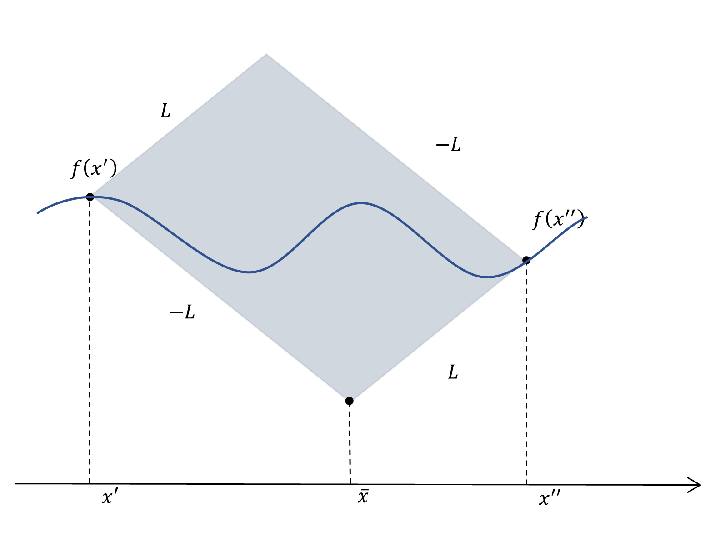
\includegraphics[width=0.8\textwidth]{Fig1.pdf}
\caption{The values of the function $f(x)$ must be inside the area highlighted by colour} \label{fig1}
\end{figure}

Also according to (\ref{f_lip}), we can write the inequality $f(x) \geq F(x)$, where the function  $F(x)$ (called the minorant) is defined according to the formula

\[
F(x) = \max\left\{f(x') - L(x-x'),f(x') + L(x-x'')\right\}, \; x\in [x', x''].
\] 

The smallest value of the minorant $F(x)$ on $[x', x'']$ coincides with the estimate of the smallest value of the function $f(x)$ on this interval. This estimate is reached at the point
\[
\overline{x} = \frac{x'+x''}{2}-\frac{f(x'')-f(x')}{2L}
\] 
and equals
\[
F(\overline{x}) = \frac{f(x')+f(x'')}{2} -L \frac{x''-x'}{2}.
\]

Lipschitz global optimization methods use this idea in their computational rules; the proof of their convergence is also based on this idea (see, e.g.,
\cite{Jones2021,PaulaviciusZilinskas2014,Sergeyev2013,Evtushenko2013}).

\subsection{The problem of dimensionality reduction} 

One of the main difficulties in solving multidimensional global optimization problems is the increase in computational cost as the dimensionality of the problem increases. This difficulty also occurs when solving Lipschitzian global optimization problems. 
For example, solving problem (\ref{f_func}) by means of the uniform grid search with a step $\epsilon$ will require performing
\[
K \approx \prod_{j=1}^N{\frac{b_j-a_j}{\epsilon}}
\]
trials. Obviously, $K$ increases exponentially with increasing $N$. It is possible to reduce the number of trials with the same requirements to the solution accuracy using the adaptive construction of a non-uniform grid in the region of parameter variation. 


A well-known approach to solving the multidimensional problem (\ref{f_func}) is to reduce it to a one-dimensional problem and then apply efficient one-dimensional global optimization algorithms (see \cite{Strongin2000,Sergeyev2013}). A well-proven approach here is to reduce the dimensionality of the problem by means of a Peano-Hilbert curve $y(x), x \in [0, 1]$.  Such a curve uniquely and continuously maps the interval $[0, 1]$ onto the hyperinterval $D$ of (\ref{f_D}), i.e., it fills the entire region $D$.


To solve the Lipschitz global optimization problem, space-filling curves can be applied as follows. If $y(x)$ is a Peano-Hilbert curve, then it follows from the continuity of the objective function $\varphi(y)$ that
\[
\min_{y \in D } \varphi(y) = \min_{x \in [0,1] } \varphi(y(x)),
\]
i.e., the original multidimensional problem (\ref{f_func}) is reduced to a one-dimensional problem.

It is known (see \cite{Strongin2000}) that if a multidimensional function  $\varphi(y), \; y \in D$,  satisfies the Lipschitz condition with the constant $L$, then the reduced one-dimensional function $\varphi(y(x)), \; x \in [0,1]$ satisfies the H{\"o}lder condition
\[
\left|\varphi(y(x'))-\varphi(y(x''))\right|\leq H\left|x'-x''\right|^{1/N}, \; x',x''\in[0,1].
\]
Here, $N$ is the dimensionality of the original problem, and the coefficient
$ H=2 L \sqrt{N+3}$.

Remark 1.  The Lipshitz condition will not be satisfied for the reduced one-dimensional function $\varphi(y(x))$. However, many one-dimensional Lipschitz optimization algorithms can be generalized to the case of H{\"o}lder function minimization. A concrete example of such a generalization is given in subsection \ref{sec_GSA}.

\begin{figure}
\center
\begin{minipage}{0.45\linewidth}
\center{\includegraphics[width=0.9\linewidth]{fig2a.jpg} }
\end{minipage}
\begin{minipage}{0.45\linewidth}
\center{\includegraphics[width=0.9\linewidth]{fig2b.jpg} }
\end{minipage}
\caption{Evolvents $y_m(x)$ with $m=4$ for dimensions $N=2$ and $N=3$.}\label{fig:Peano}
\end{figure}   

Remark 2. The theoretical Peano-Hilbert curve $y(x)$ is defined as a limiting object. Numerical algorithms use evolvents $y_m(x)$, that approximate the true curve with a given density level $2^{-m}$, which depends on the required search accuracy. Efficient schemes for computing several types of evolvents are described in detail in \cite{Sergeyev2013}. For illustration, Fig.~\ref{fig:Peano} shows graphs corresponding to the evolvents $y_m(x)$ with density $m=4$ for dimensions $N=2$ and $N=3$.

\subsection{The problem of discrete parameters}
\label{sec_discr} 

Of particular interest are problems where some of the parameters can assume values from a predetermined finite set, since it is more difficult to construct estimates of the optimum for these problems than for problems with continuous parameters. Many publications address the methods for solving mixed-parameter problems (see, for example, reviews \cite{Burer2012,Boukouvala2016}). Known deterministic methods for solving problems of this class are centered on solving linear or convex problems \cite{Lee2012}. It is suggested that complex multiextremal problems should be solved using heuristic approaches \cite{Belotti2013}. 

We have proposed and implemented a new deterministic approach to solving problems with mixed parameters; here we give a brief description of it. 
Let the objective function of the problem depend on two parameter vectors: vector $y$, which belongs to the hyperinterval $D$, and vector $u$, which has a finite (and not very large) set of possible values, i.e.
\begin{gather}\label{problem_i}
\min{\left\{ \varphi(y,u) : y\in D \right\}},\\
D=\left\{a_j \leq y_j \leq b_j, \; 1\leq j \leq N \right\}.\nonumber
\end{gather}

Such finite sets of values can characterize many possible combinations of categorical hyperparameters of the machine learning algorithm under study. A typical example is the support vector machine, whose performance is influenced by the continuous regularization parameter $C$ and the kernel coefficient $\gamma$. In this case, the type of kernel function is chosen from a finite set of variants (e.g., polynomial function, radial basis function, sigmoid, etc.). 
%Целочисленные параметры = непрерывные параметры с округлением, добавить комментарий об этом?

Let us number all the different combinations of categorical parameters with integers $s, 1\leq s \leq S$, i.e., let us assign a vector $u_s$ to each number $s$. Then the problem under consideration can be written in the form
\begin{gather}\label{problem_is}
 \min_{s\in\{1,...,S\}}\left[\min{\left\{ \varphi(y,u_s) : y\in D \right\}}\right].
\end{gather}

Using a dimensionality reduction scheme with Peano curves $y(x), x\in [0,1]$,  we can assign to each minimization problem on $y$ a one-dimensional minimization problem
\[
 \min{\left\{ \varphi(y(x),u_s): x \in [0,1] \right\}}, s \in \{1,...,S\}.
\]

Let us now consider the mapping
\[
Y(x)=y(x-E(x)), \; x\in[0,S],
\]
which translates any point of the interval $[0,S]$ to the region $D$ (the notation $E(x)$ corresponds to the integer part of the number $x$) and define the function
\[
f(x) = \varphi(Y(x),u_{E(x)+1}), x\in[0,S],
\]
which has, generally speaking, discontinuities at integer points $x_i = i, 1 \leq i \leq S-1$.
Therefore, the values $z_i = f(x_i)$ at these points will be considered undefined and will not be used in the algorithm.
%, а значения индекса -- равным 0, т.е. $\nu(x_i) = 0$.

Using the introduced notations, we can reformulate the original problem as
\begin{equation}\label{problem_is1}
\min \left\{f(x): x \in [0,S] \right\}.
\end{equation}

Applying the global search algorithm to the solution of problem (\ref{problem_is1}), we will find the solution of problem (\ref{problem_i}). In this case, the main part of trials will be carried out in the $s$-th subproblem, whose solution corresponds to the solution of the original problem (\ref{problem_i}). In the other subproblems, only a small part of trials will be carried out, since the solutions of these subproblems are locally optimal with respect to the solution of the $s$-th subproblem.

\section{iOpt framework} 
\label{sec_iOpt}

The iOpt framework of intelligent optimization methods is designed to select optimal (in a given metric) values of parameters of complex objects and processes, especially in artificial intelligence and machine learning methods. The framework allows fine-tuning of parameters of models and methods used in applied research in various fields of science.  The iOpt framework was designed in the Python programming language using its standard library. To use the framework, you need to have the Python interpreter version 3.8 or higher installed. The framework is open source and is available at \url{https://github.com/aimclub/iOpt}.
\textcolor[rgb]{1,0,0}{The general structure of the framework is shown in Fig. \ref{fig_iOpt}. 
Description of the main algorithms used in iOpt is given in the following sections.
}
\begin{figure}[t]
\centering
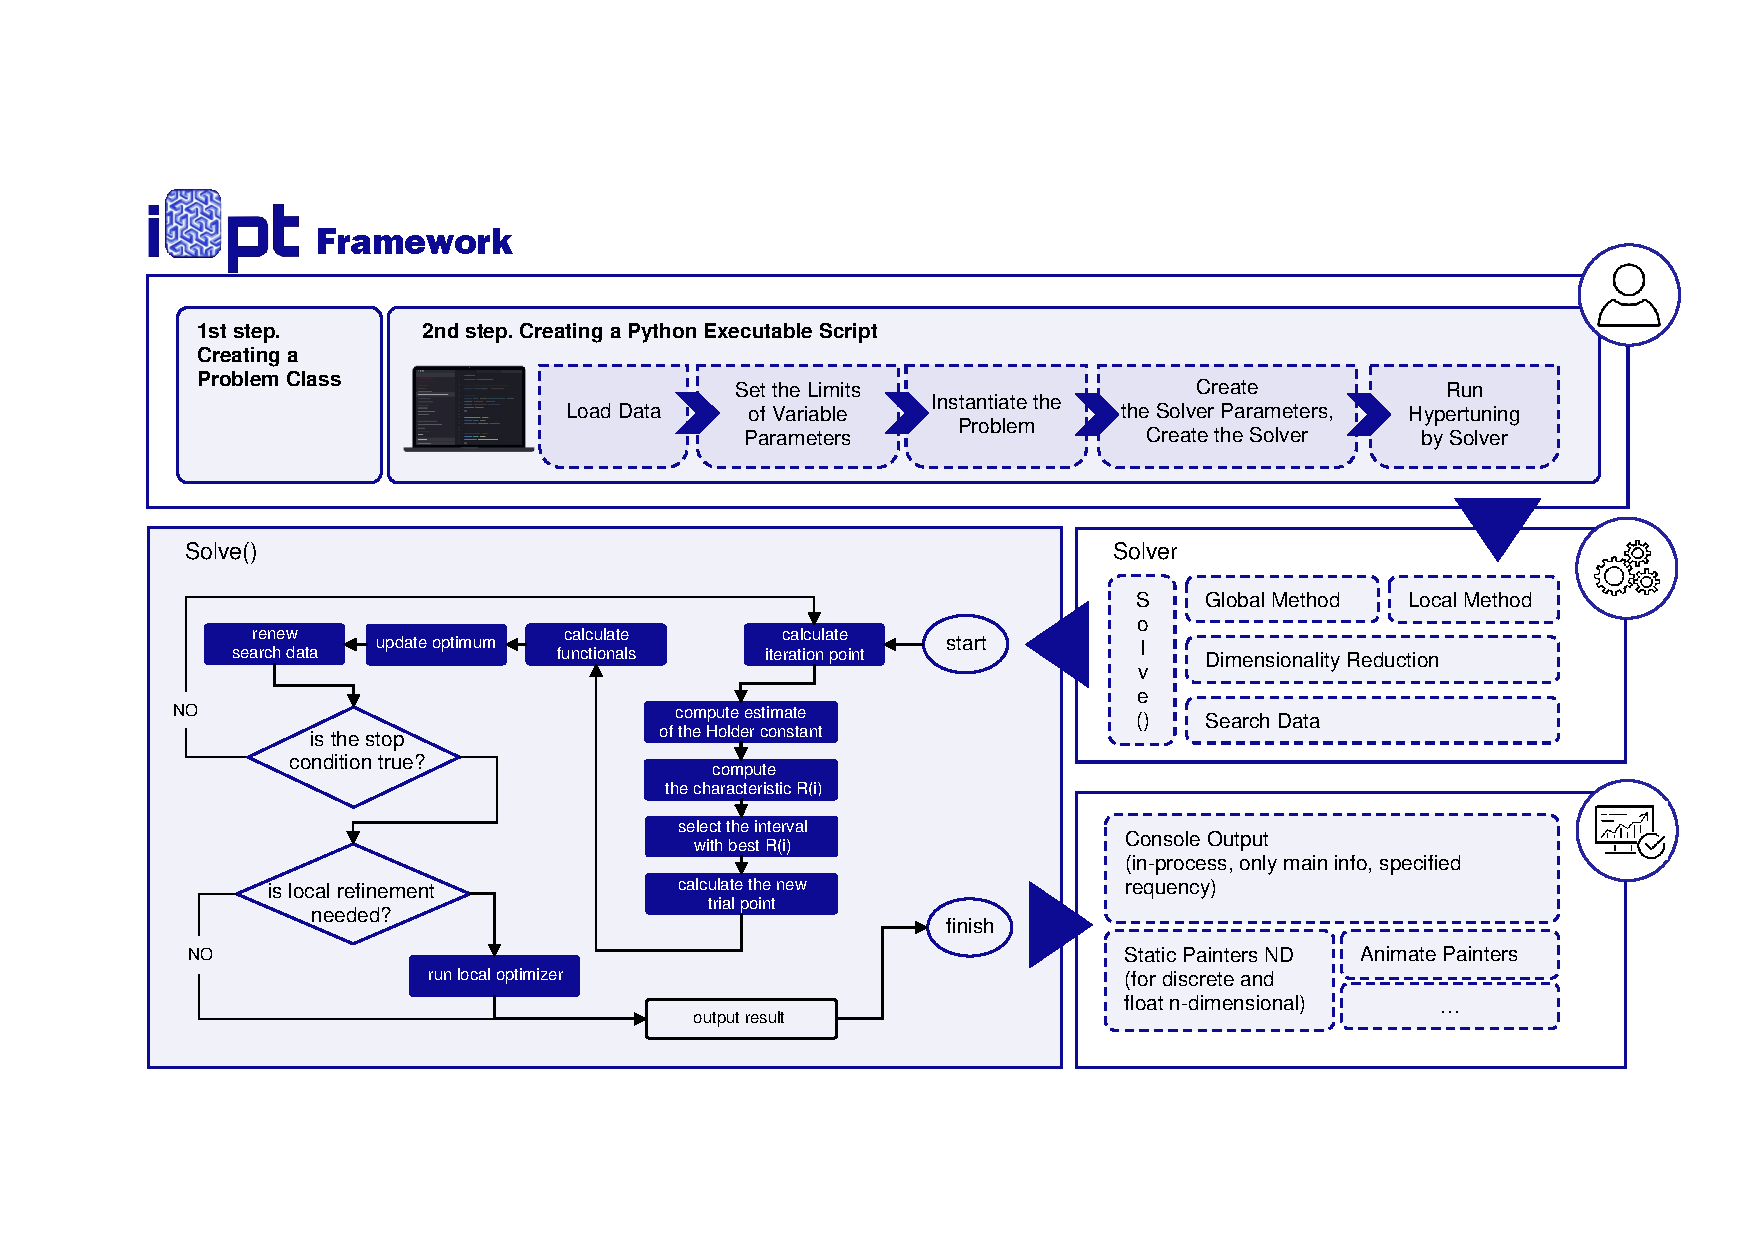
\includegraphics[width=1.0\textwidth]{scheme.pdf}
\caption{iOpt general structure} \label{fig_iOpt}
\end{figure}


The iOpt framework can be used to develop specialized decision support systems for solving the tasks of selecting optimal parameters for complex models or methods. The application area of the framework is focused on the hyperparameter tuning tasks, since this class of tasks involves the problems of multiextremality of the optimization criterion and the lack of a formula-based description of the model under study (a ``black box'' type model).


\subsection{Global search algorithm}
\label{sec_GSA}

The algorithmic core of the iOpt framework is an information-statistical global search algorithm for solving problems of the form (\ref{f_func}), (\ref{f_D}). This algorithm assumes the construction of a sequence of points $y^i$,  at which search trials are performed, i.e., the values of the objective function $z^i = \varphi(y^i)$ are computed. According to the dimensionality reduction scheme used, conducting a trial implies computing $y^i=y(x^i)$, so the result of the trial will be a set of values $(x^i, y^i=y(x^i), z^i = \varphi(y^i))$. 
It is convenient to represent the search information accumulated after conducting $k$ trials as a set in which the corresponding entries are renumbered (by the lower index) in ascending order of $x$, i.e., as a set 
\begin{equation}\label{omega}
\Omega_k = \left\{  (x_i, y_i=y(x_i), z_i = \varphi(y_i)): 1 \leq i \leq k  \right\},	
\end{equation}
where $x_1 < x_2 < ... < x_k$.

The main idea of the global search algorithm is as follows. Let $k \geq 2$ trials be conducted in the search process and the search information $\Omega_k$ from (\ref{omega}) is obtained. To select the point of the next trial for each search interval $(x_{i-1},x_i), 1<i\leq k$, its characteristic is calculated according to the following formula
\begin{equation}\label{R}
R(i) = \Delta_i + \frac{(z_i-z_{i-1})^2}{(r\mu)^2\Delta_i}-2\frac{z_{i-1}+z_i}{r\mu}.	
\end{equation}

Here,  $r>1$ is the algorithm parameter, $\Delta_i=(x_i-x_{i-1})^{1/N}$.  The value $\mu$ is the lower estimate of the H\"older constant of the objective function computed using the search information from (\ref{omega}) by the formula
\begin{equation}\label{mu}
\mu = \max_{1<i\leq k}\frac{\left|z_i-z_{i-1}\right|}{\Delta_i},
\end{equation}
and in case when formula (\ref{mu}) gives the value $\mu=0$, the value $\mu=1$ is used.

A new trial is performed at the point $x^{k+1}$ that belongs to the interval
with the largest characteristic. If the right point of this interval has the number $t$ in the set $\Omega_k$, then the formula for calculating $x^{k+1}$ will look as follows:
\begin{equation}\label{xk1}
x^{k+1} = \frac{x_t+x_{t-1}}{2}- \frac{\mathrm{sign}(z_t-z_{t-1})}{2r} \left(\frac{\left|z_t-z_{t-1}\right|}{\mu}\right)^N.   
\end{equation}

Algorithm \ref{alg_GSA} shows the pseudo code of the Global Search Algorithm. The input data of the algorithm are the objective function $\varphi(y)$ and the search region $D$ from (\ref{f_func}) and (\ref{f_D}), the algorithm parameter $r>1$, the minimum search accuracy $\epsilon > 0$, and the maximum allowable number of trials $K_{max}$. The output parameter of the algorithm is an estimate of the global minimum point $y_{min}$. Additional output parameters can include the value of the function at the minimum point $\varphi(y_{min})$ and the number of trials $k$.

\begin{algorithm}
\LinesNumbered
 \KwIn{$\varphi(y), D, r, \epsilon, K_{max}$}
 \KwOut{$y_{min}$}
 Initialize $k=2$, $t=2$, $\Omega_k= \left\{ (x_1=0, y_1=y(x_1), z_1=\varphi(y_1)), (x_2=1, y_2=y(x_2), z_2=\varphi(y_2)) \right\}$\\
 \While{ $\Delta_t \geq \epsilon$ and  $k \leq K_{max}$}{
  Compute the estimate of the H\"older constant $\mu$ according to (\ref{mu})\\
	\For{$i=1$ \KwTo $k$}{
	Compute the characteristic $R(i)$ according to (\ref{R})\\
	}
	Determine the number $t$, for which $R(t) = \max \left\{ R(i), 1 \leq i \leq k \right\}$
	
	Compute the new trial point $x^{k+1}$ according to (\ref{xk1})
	
	Perform a new trial at the point $x^{k+1}$
	
	Add $(x^{k+1}, y^{k+1}, z^{k+1})$ to the set $\Omega_k$
	
  $k = k + 1$\\
 }
 $l = \arg \min \left\{ z_i, 1 < i \leq k \right\}$\\
 $y_{min} = y_l$, \\ 
 \KwRet{$y_{min}$}
 \caption{Global search algorithm}\label{alg_GSA}
\end{algorithm}

The theory of algorithm convergence as well as some of its modifications are presented in \cite{Strongin2000}.

\subsection{GSA for the problems with categorical parameters}
\label{sec_mGSA}

Let us consider the case when the algorithm to be tuned has both continuous and categorical parameters.  In this case, the categorical parameters can be assigned integer values, and the problem can be reduced to the formulation (\ref{problem_is1}).
Since the solution of problems with partially integer parameters in accordance with the scheme described in Section \ref{sec_discr} implies the solution of problem (\ref{problem_is1}) with a discontinuous objective function, a modification of the algorithm that takes this feature into account is required.

For this purpose, we introduce the classification of points from the search region using a special index $\nu_i=\nu(x_i)$. We will assume the indices of integer points $x_i = i, 0\leq i \leq S$, to be equal to zero, i.e. $\nu(x_i) = 0$. For all other values of $x\in(i,i+1),  0 \leq i < S$, we will assume the index value to be equal to unity, i.e.  $\nu(x) = 1$. Then the result of the trial at some point $x^j\in[0,S]$  will be the set of values $(x^j, \nu^j=\nu(x^j), y^j=y(x^j), z^j = \varphi(y^j))$. In the case of  $\nu^j=0$, the value of $z^j$ will be considered undefined.

The general computational scheme outlined as Algorithm \ref{alg_GSA} will remain the same. The modifications will consist of the following.

1. At the initialization stage, the values $(x^i = i, \nu^i=0, y^i=y(x^i), z^i)$, $ i, 0\leq i \leq S$, i.e., the boundary points of the intervals $(x_{i-1},x_i), 1<i\leq S$, are entered into the set $\Omega_k$ containing the search  information. 
After that, trials are carried out at arbitrary internal points (e.g., midpoints) of the intervals $(x_{i-1},x_i), 1<i\leq S$; the trial results are also added to the search information. Thus, after initialization, the set $\Omega_k$ will contain $k=2S+1$ elements.

2. The computation of the estimate of the H\"older constant $\mu$ according to formula (\ref{mu}) must be performed only for intervals for which $\nu(x_i) = \nu(x_{i-1}) = 1$, i.e., when the values $z_i$ and $z_{i-1}$ are determined.

3. The computation of the characteristic of the search interval $(x_{i-1},x_i), 1<i\leq k$, is performed according to the following rules:
\begin{gather}\label{R_int}
R(i) = \Delta_i + \frac{(z_i-z_{i-1})^2}{(r\mu)^2\Delta_i}-2\frac{z_{i-1}+z_i}{r\mu}, \; \mathrm{if} \; \nu(x_i) = \nu(x_{i-1}) = 1, \nonumber \\ 
R(i) = 2\Delta_i-4\frac{z_i}{r\mu}, \; \mathrm{if} \;  \nu(x_i) = 1, \nu(x_{i-1}) = 0, \nonumber \\ 
R(i) = 2\Delta_i-4\frac{z_{i-1}}{r\mu}, \; \mathrm{if} \;  \nu(x_{i-1}) = 1, \nu(x_{i}) = 0. \nonumber
\end{gather}

Note that the algorithm will not produce intervals whose both boundary points have undefined function values, i.e., $\nu(x_i) = \nu(x_{i-1}) = 0$.

4. The new trial point $x^{k+1}$ will be calculated as follows:
\begin{gather}\label{xk1_int}
x^{k+1} = \frac{x_t+x_{t-1}}{2}- \frac{\mathrm{sign}(z_t-z_{t-1})}{2r} \left(\frac{\left|z_t-z_{t-1}\right|}{\mu}\right)^N, \; \mathrm{if} \; \nu(x_i) = \nu(x_{i-1}) = 1, \nonumber \\    
x^{k+1} = \frac{x_t+x_{t-1}}{2} , \; \mathrm{if} \; \nu(x_i) \neq \nu(x_{i-1}). \nonumber
\end{gather}

Here, $t$ is the number of the search interval that has the maximum characteristic.

We note again that the characteristic $R(i)$ quantifies the possibility of finding a point $x^*$, which is the inverse image of the global optimizer $y^* = y(x^*)$, within the considered interval $(x_{i-1},x_i)$.

\section{Numerical experiments}
\label{sec_exp}

In this section, we present experimental results that demonstrate the effectiveness of the developed framework for a number of HPO problems. First, we describe in detail the setup of the computational experiment. Then, the results of comparing the iOpt framework with several well-known frameworks widely used for hyperparameter tuning in machine learning methods are presented. The section closes with conclusions and a discussion of the results.

\subsection{Experimental setup}

\textbf{Datasets.} 
We used for our experiments fifteen datasets from the UCI repository \cite{UCI}, which covers a large number of areas. Datasets from this repository are quite often used to test the correct operation of hyperparameter tuning algorithms \cite{Joy2020,Wang2021,Wu2023}. We selected the datasets to ensure that the data contained in them were described by both numerical and categorical attributes. Note that most of the datasets were unbalanced and the data presented in the datasets were adapted for the classification task.  The characteristics of the datasets used are presented in Table \ref{tab:1}.


\begin{table}[ht]
\caption{The datasets used in the experiments}
\label{tab:1}
\begin{tabular}{lcccccc}
\hline
Name                                                            & Num   & Attributes & Int & Float & Categorical & Classes \\ \hline
Balance                                                         & 625   & 4          & 4   & 0     & 0           & 3       \\
Bank Marketing                                                  & 45211 & 20         & 6   & 4     & 10          & 2       \\
Banknote                                                        & 1372  & 4          & 0   & 4     & 0           & 2       \\
Breast Cancer                                                   & 569   & 9          & 9   & 0     & 0           & 2       \\
CarEvaluation                                                   & 1728  & 6          & 0   & 0     & 6           & 4       \\
CNAE9                                                           & 1080  & 856        & 856 & 0     & 0           & 9       \\
Credit Approval                                                 & 690   & 15         & 0   & 6     & 9           & 2       \\
Digits                                                          & 5620  & 64         & 64  & 0     & 0           & 10      \\
Ecoli                                                           & 336   & 7          & 0   & 7     & 0           & 8       \\
Parkinsons                                                      & 197   & 22         & 0   & 22    & 0           & 2       \\
Semeion                                                         & 1593  & 256        & 256 & 0     & 0           & 10      \\
\begin{tabular}[c]{@{}l@{}}Statlog \\ Segmentation\end{tabular} & 2310  & 19         & 1   & 18    & 0           & 7       \\
Wilt                                                            & 4889  & 5          & 0   & 5     & 0           & 2       \\
Zoo                                                             & 101   & 16         & 16  & 0     & 0           & 7       \\ \hline
\end{tabular}
\end{table}

\textbf{Classification algorithms.} We performed hyperparameter tuning for three types of classification algorithms on all datasets.
\begin{enumerate}
	\item XGBoost is one of the tree ensemble construction methods, which is an efficient implementation of gradient boosting over decision trees \cite{XGBoost2016}. The main advantages of the algorithm include a smart penalty mechanism, proportional reduction of leaf nodes, and automatic feature selection. It is known that the performance of an algorithm and its predictive ability depend significantly on the correct tuning of hyperparameters. The implementation of the method is based on the widely used XGBoost library.
 \item Multi-Layer Perceptron (MLP), a fully connected artificial neural network, is a supervised learning algorithm that forms a function $f : R^m \to R^o$, where $m$ is the number of input attributes, and $o$ is the output dimensionality of the network \cite{GARDNER19982627}. Using this method, it is possible to form the function f as a universal nonlinear approximator for the classification and regression problem. In the framework of this study, we will consider the multilayer perceptron for the task of attributing an object to a particular class.
 \item Support Vector Classification (SVC) is a support vector method for the classification problem \cite{SVC}. The main purpose of this algorithm is to find the equation of a separating hyperplane $\omega_0 + \sum_{i=1}^n \omega_i x_i=0$ in the space $R^n$ that separates classes in some optimal way. To improve the predictive ability of the algorithm, a method for constructing a nonlinear classifier was proposed by switching from scalar products to arbitrary kernels, which allows the construction of nonlinear separators. An implementation of the SVC method from the scikit-learn library was used to investigate the capabilities of HPO algorithms.

\end{enumerate}

The tunable hyperparameters of the above algorithms and their search region are listed in Table \ref{tab:2}.

\begin{table}[ht]
\caption{Tunable hyperparameters of machine learning algorithms.}
\label{tab:2}
\begin{tabular}{lccc}
\hline
Method  & Parameters & Parameter type & Parameter range \\ \hline
\multirow{7}{*}{XGBoost} & n\_estimators        & Int           & {[}10, 200{]}                                                          \\
                         & max\_depth           & Int           & {[}5, 20{]}                                                            \\
                         & min\_child\_weight   & Int           & {[}1, 10{]}                                                            \\
                         & Gamma                & Float         & {[}0.01, 0.6{]}                                                        \\
                         & Subsample            & Float         & {[}0.05, 0.95{]}                                                       \\
                         & colsample\_bytree    & Float         & {[}0.05, 0.95{]}                                                       \\
                         & learning\_rate       & Float         & {[}0.001, 0.1{]}                                                       \\ \hline
\multirow{3}{*}{\begin{tabular}[c]{@{}l@{}}Support \\ Vector   \\ Classification \\ (SVC)\end{tabular}} &
  Gamma &
  Float &
  {[}$10^{-9}$, $10^{-6}${]} \\
                         & C                    & Int           & {[}$10^1$,$10^{10}${]}                     \\
                         & Kernel               & Categorial    & \begin{tabular}[c]{@{}l@{}}\{‘poly’, ‘rbf’,\\ ‘sigmoid’\}\end{tabular} \\ \hline
\multirow{4}{*}{\begin{tabular}[c]{@{}l@{}}Multi-layer   \\ Perceptron \\ (MLP)\end{tabular}} &
  Activation &
  Categorial &
  \begin{tabular}[c]{@{}l@{}}\{'identity', \\ 'logistic', \\ 'tanh', 'relu'\}\end{tabular} \\
                         & hidden\_layer\_sizes & Int           & {[}2, 30{]}                                                            \\
                         & max\_iter            & Int           & {[}100, 700{]}                                                         \\
                         & Solver               & Categorial    & \begin{tabular}[c]{@{}l@{}}\{'lbfgs', 'sgd', \\ 'adam'\}\end{tabular}  \\ \hline
\end{tabular}
\end{table}

\textbf{Evaluation Metrics.} To evaluate the quality of machine learning methods on the considered datasets, it is necessary to determine the metrics. In view of the peculiarities of datasets, namely their unbalanced nature and the different number of classes in different datasets, the use of a single metric would result in a biased evaluation. Therefore, we used the following set of metrics:
\begin{itemize}
	\item Accuracy is a metric describing the overall prediction accuracy of the method across all classes. It is most visible in the case when each class is equally important and the dataset shows a balance of classes \cite{Metric1}. This metric has been applied when working with the datasets Optical Recognition of Handwritten Digits, Bank Marketing, CNAE9, Statlog Segmentation, Semeion Handwritten Digit;
 \item Binary F1 -- F1 score is adapted for binary classification tasks, with the predominance of one class over another in the dataset \cite{Chicco2020}. This metric is suitable for analyzing Breast Cancer Wisconsin, Credit Approval, Parkinsons, Banknote authentication, Wilt datasets; 
 \item Macro F1 -- F1 score is suitable for tasks with a large number of unbalanced classes \cite{Metric2}. The datasets Protein Localization Sites (Ecoli), Balance Scale Weight \& Distance, Zoo, Car Evaluation, Turkiye Student Evaluation have this particular feature.

\end{itemize}

\textbf{HPO algorithms.} The hyperparameters of machine learning methods were tuned using the iOpt framework developed by us, and also using the well-known frameworks Optuna \cite{optuna} and HyperOpt \cite{hyperopt}.

Optuna is an automatic hyperparameter optimization software environment specifically designed for optimizing hyperparameters of machine learning algorithms. Several methods for selecting test points, which are referred to as \textit{samplers} within this framework, are available in Optuna.  In the study, we used the following hyperparameter search options:
\begin{enumerate}
	\item Optuna(random) will perform a random search. For each hyperparameter, a distribution is specified, from which its value is selected.
	\item Optuna(tpe) is a sampler based on the Tree-structured Parzen Estimator algorithm \cite{NIPS2011_86e8f7ab}. On each trial, for each parameter, TPE fits one Gaussian Mixture Model (GMM) $l(x)$ to the set of parameter values associated with the best objective values, and another GMM $g(x)$ to the remaining parameter values. It chooses the parameter value x that maximizes the ratio $l(x)/g(x)$.
	\item Optuna(cmaes) is an algorithm based on CMA-ES (Lightweight Covariance Matrix Adaptation Evolution Strategy) \cite{cmaes2015}. The CMA-ES is a stochastic method for real-parameter optimization of non-linear, non-convex functions. The algorithm derived from intuitive concepts and from requirements of non-linear, non-convex search in continuous domain.
	\item Optuna (nsgaii) is a sampler based on the Nondominated Sorting Genetic Algorithm II,  which is a well known, fast and elitist multi-objective genetic algorithm \cite{nsgaii2013}.

\end{enumerate}


Hyperopt framework is a Python library for optimization over complex search spaces, which may include real-valued, discrete, and conditional dimensions. As with Optuna, Hyperopt has different options for finding hyperparameter values. There are currently three algorithms implemented in Hyperopt: Random Search, Tree of Parzen Estimators (TPE) and Adaptive TPE. We used the computation variant with the TPE algorithm implementation -- Hyperopt(tpe) \cite{NIPS2011_86e8f7ab}.

When using the iOpt framework, we applied a variant of computation in which the available resource was divided into portions by the number of trials. Most of the trials (75\%) were performed using the global search algorithm (see Section \ref{sec_iOpt}), while in the remaining trials we used the local method to refine the solution found \cite{Kelley}.

\subsection{Results and discussion}

Computational experiments were performed on the computing nodes of the Lobachevsky supercomputer (Intel Xeon Silver 4310T CPU @ 2.30GHz, 64Gb RAM, Linux CentOS 7). We used the following versions of frameworks for the experiments: iOpt 0.2.22, Optuna 3.1.1, Hyperopt 0.2.7. All runs were performed using Python version 3.11.3.

In one experiment on hyperparameter tuning, we ran 200 search trials with each method. Due to the stochastic nature of the Optuna and Hyperopt algorithms, we ran them 10 times and calculated both the average and worst values of the objective  metric. For iOpt, we ran it once because the global search algorithm is deterministic and the average, worst and best case values are the same.

Figures \ref{fig_res_1} and \ref{fig_res_2} show the values of the classification metrics of the SVC algorithm in the worst and average case, respectively. As can be seen, when optimizing the hyperparameters of the SVC algorithm on the Banknote, CNAE-9, Statlog Segmentation, and Wilt datasets, the iOpt framework has demonstrated the best results.

\begin{figure}
\centering
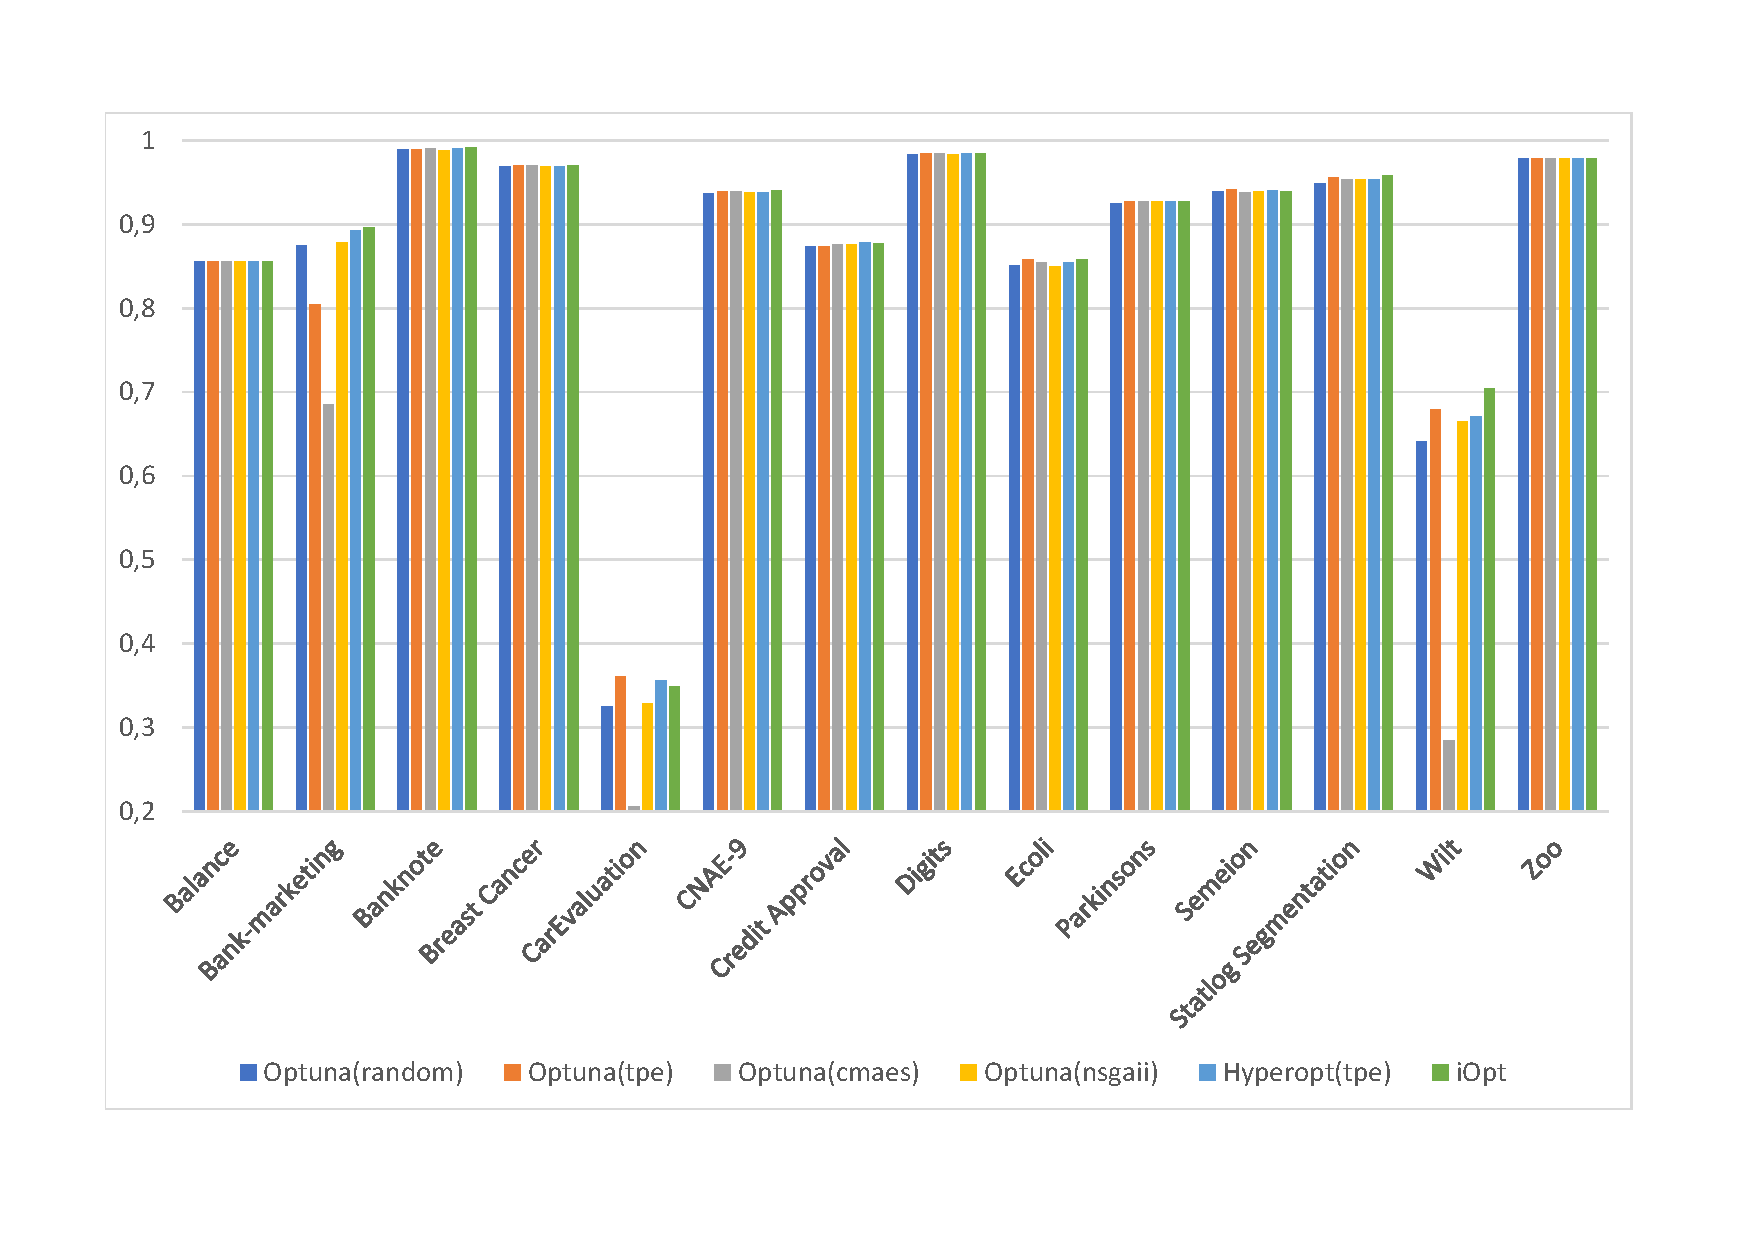
\includegraphics[width=0.85\textwidth]{SVC_1.pdf}
\caption{Values of the optimized metrics for the SVC algorithm, obtained in the worst case} \label{fig_res_1}
\end{figure}

\begin{figure}
\centering
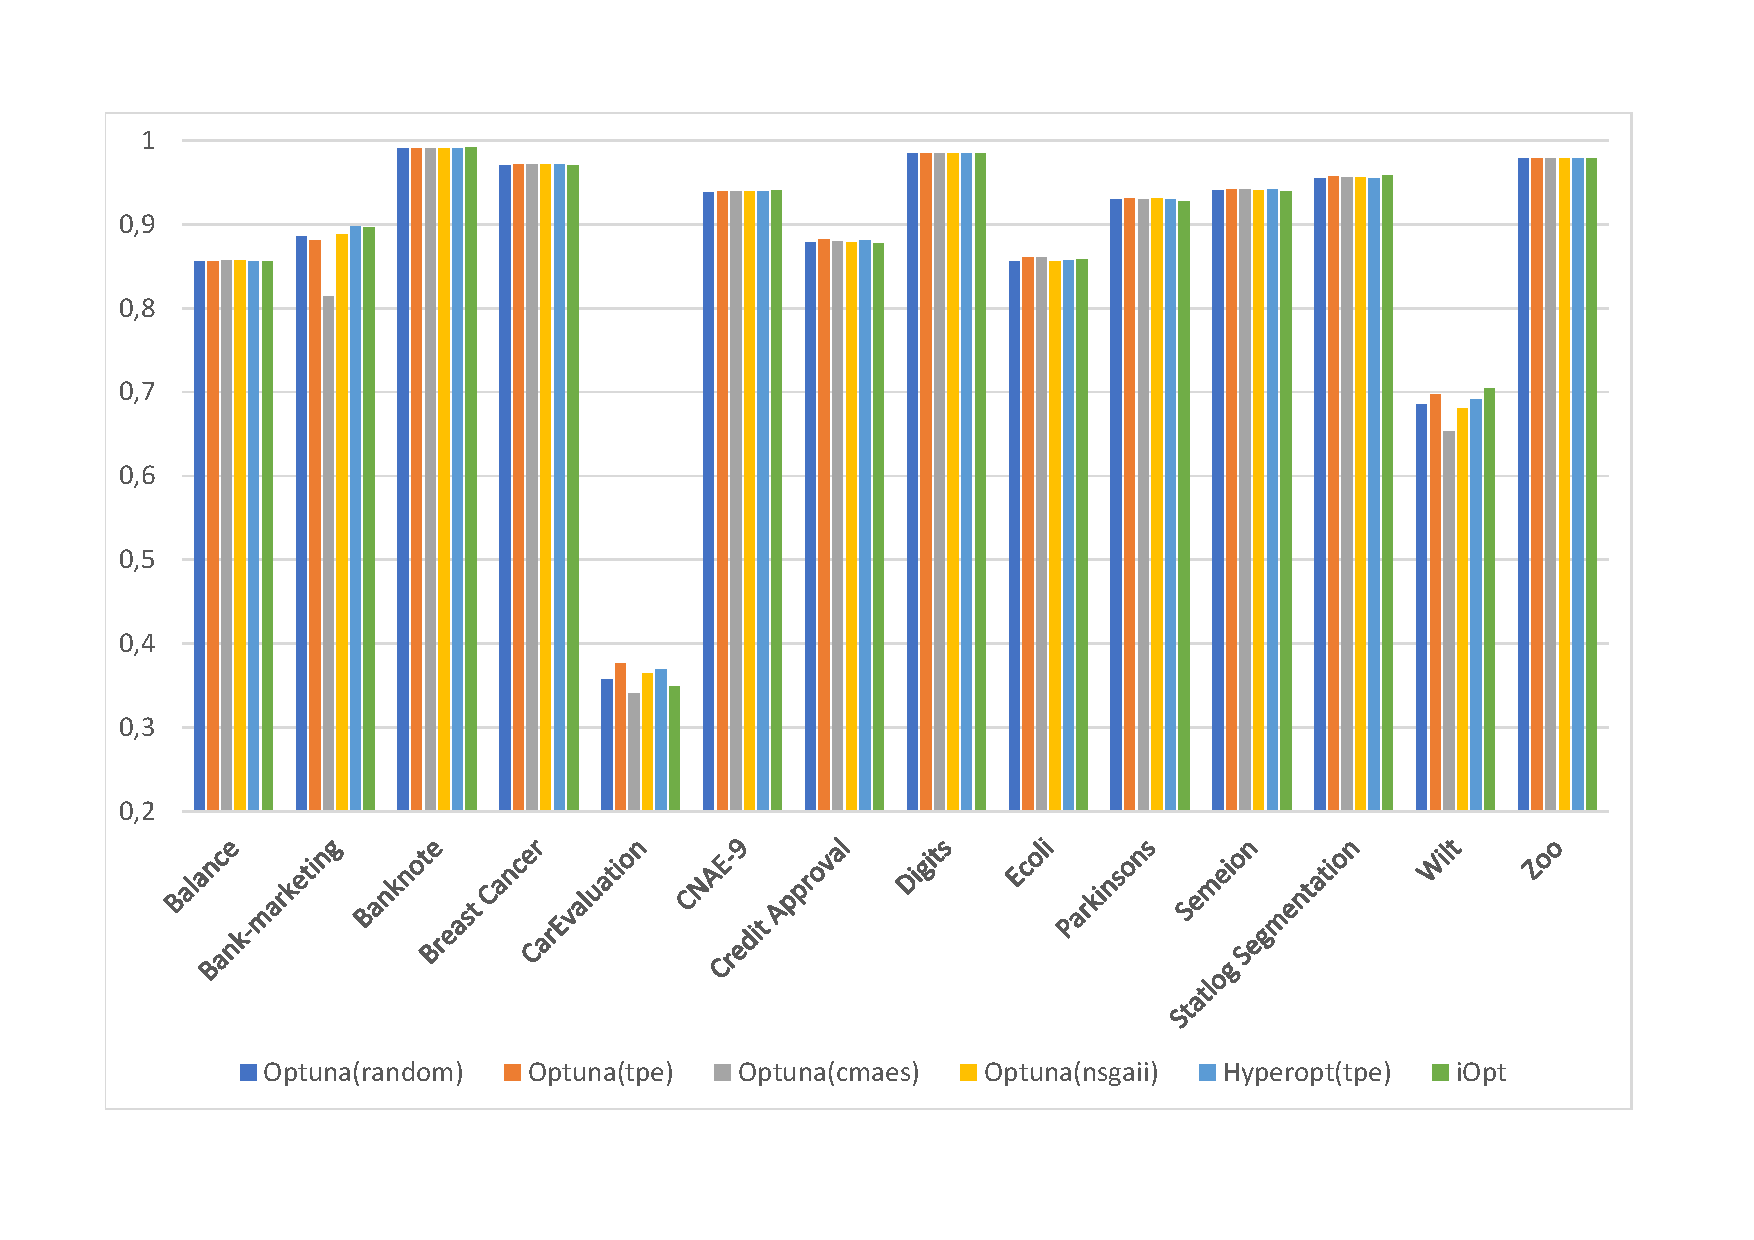
\includegraphics[width=0.85\textwidth]{SVC_2_avg.pdf}
\caption{Values of optimized metrics for the SVC algorithm averaged over 10 runs} \label{fig_res_2}
\end{figure}


On the CarEvaluation, Credit Approval, Ecoli, Parkinsons, and Semeion datasets, the best values of the metrics on average were obtained with the Optuna (tpe). On the datasets Balance, Breast Cancer, Digits, on average the Optuna(cmaes) performed well. The Hyperopt(tpe) performed better than the others on the Bank-marketing dataset. In the case of the Zoo dataset, all optimization algorithms showed the same results.

It is especially worth noting that the algorithms implemented in both Optuna and Hyperopt contain random parameters; as a consequence, the best values of the objective metric are not guaranteed for a single run. 

This fact is illustrated by Fig. \ref{fig_res_1}. The iOpt framework additionally performed better on the Bank-marketing, Banknote, CNAE-9, Statlog Segmentation, and Wilt datasets. Thus on 9 out of 14 datasets the iOpt framework showed better values of the objective metric compared to the Optuna and Hyperopt frameworks.


\begin{figure}
\centering
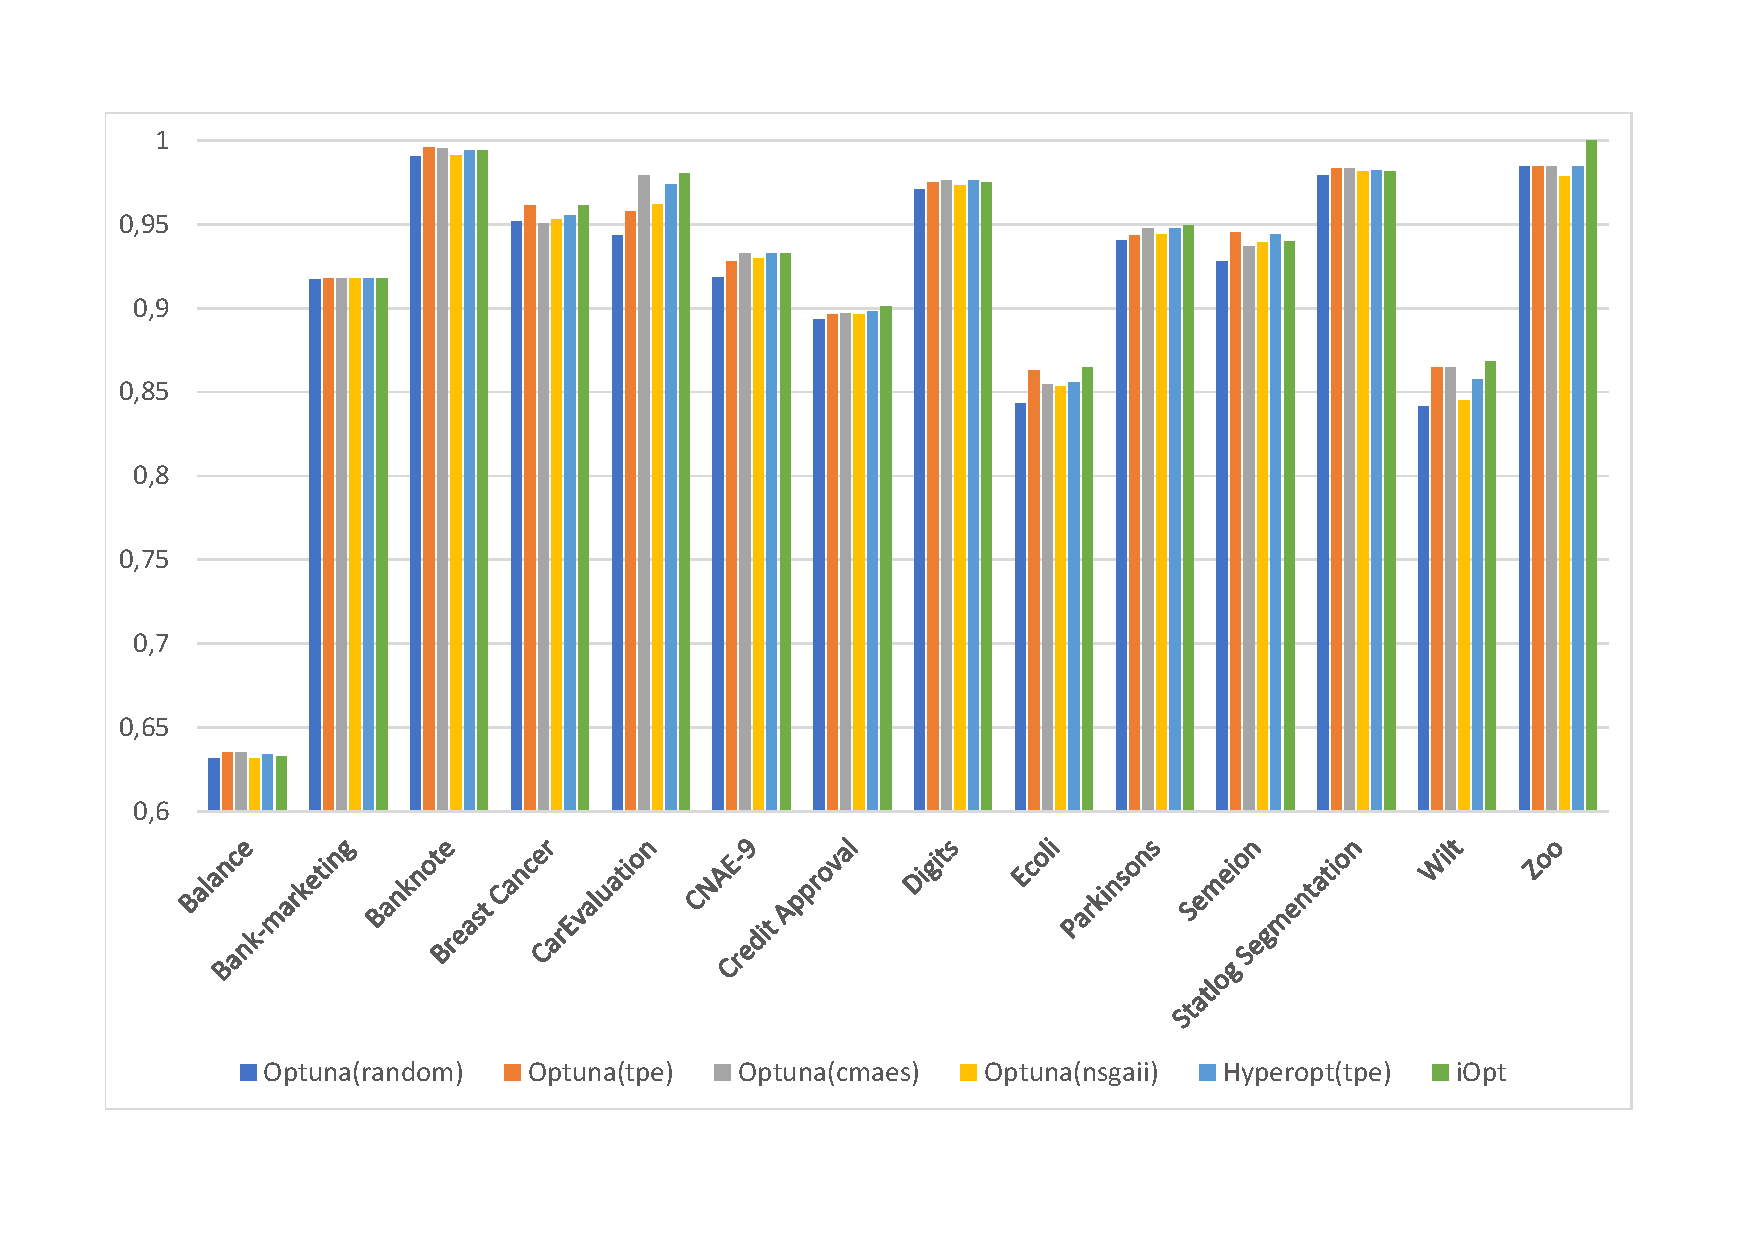
\includegraphics[width=0.85\textwidth]{XGBoost_1.pdf}
\caption{Values of the optimized metrics for the XGBoost algorithm, obtained in the worst case} \label{fig_res_3}
\end{figure}

\begin{figure}
\centering
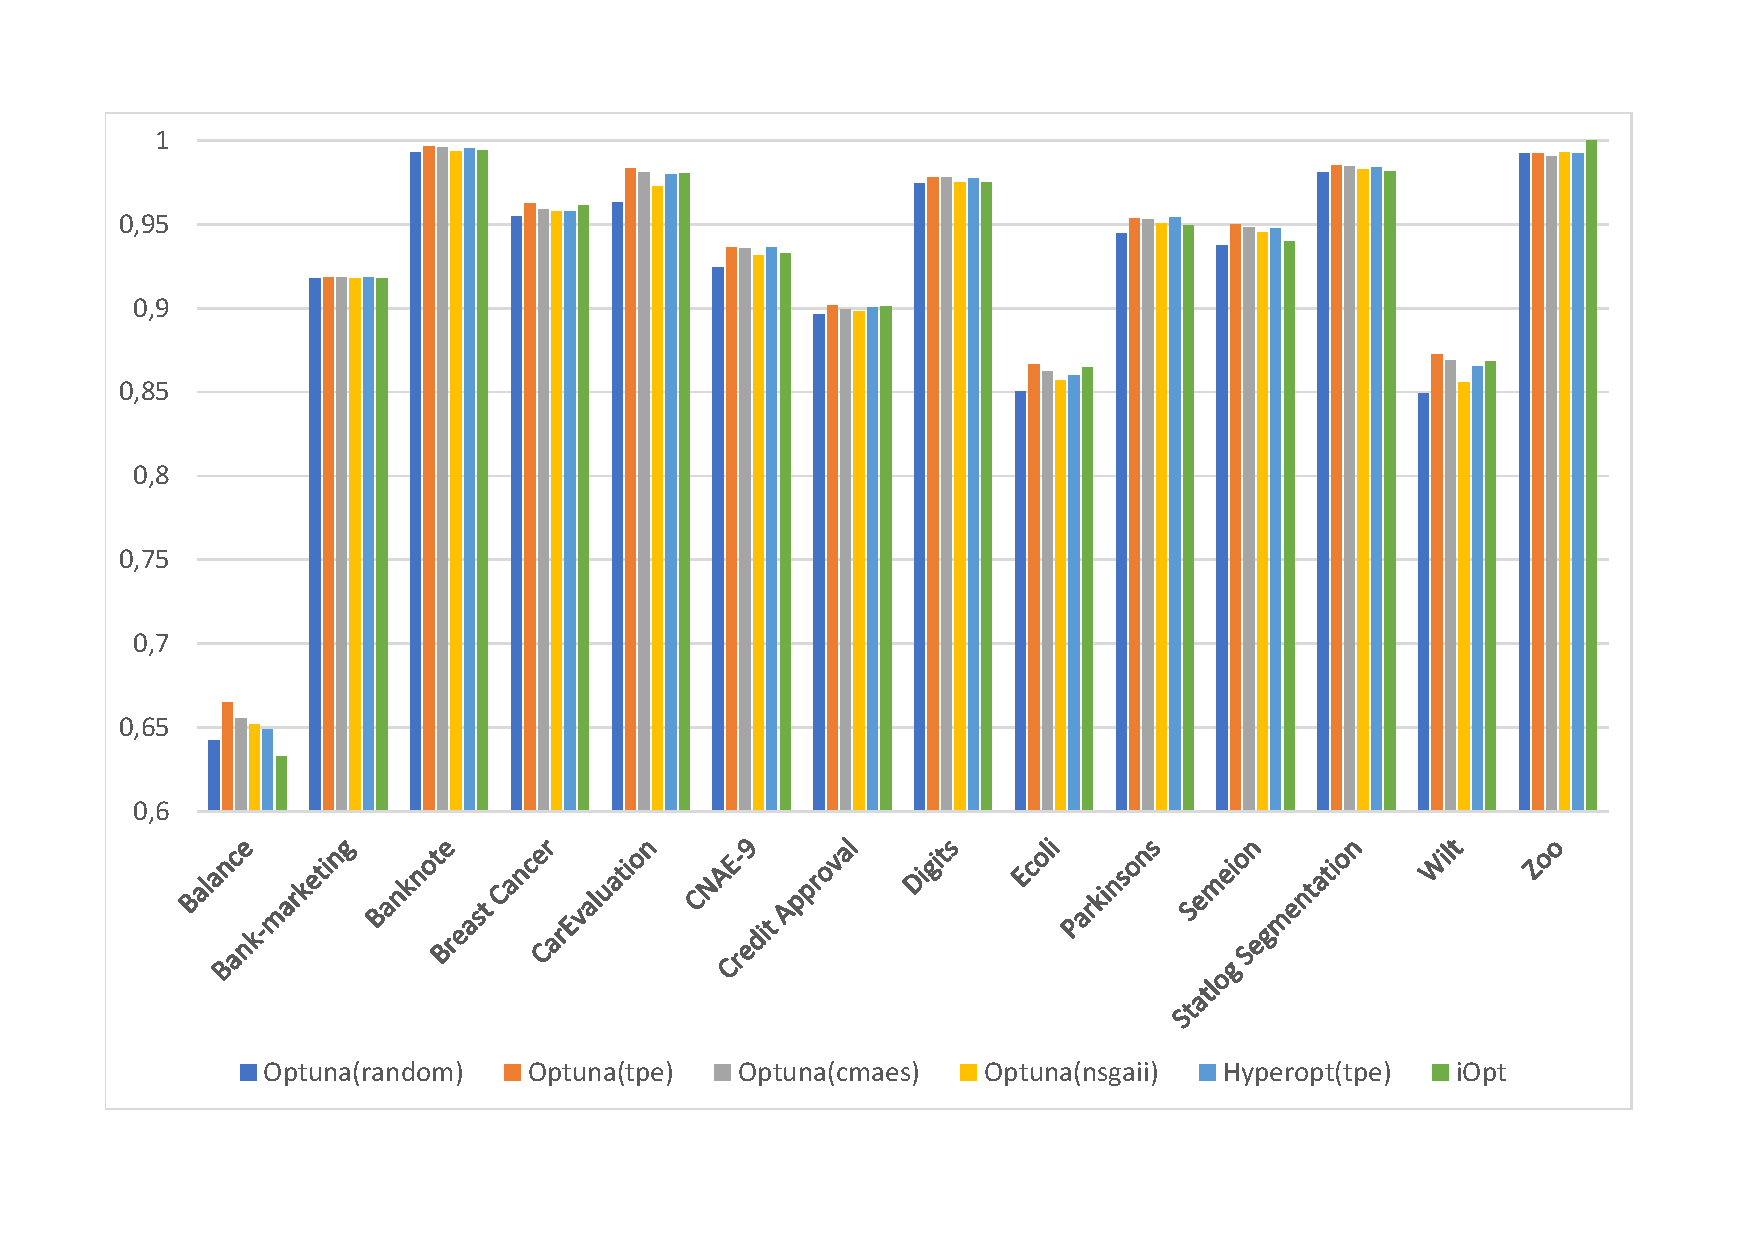
\includegraphics[width=0.85\textwidth]{XGBoost_2_avg.pdf}
\caption{Values of optimized metrics for the XGBoost algorithm averaged over 10 runs} \label{fig_res_4}
\end{figure}

Figures \ref{fig_res_3} and \ref{fig_res_4} show the value of classification metrics of the XGBoost algorithm in the worst and average case, respectively. In the case of optimizing the hyperparameters  of the XGBoost algorithm, the iOpt framework showed better results on the CarEvaluation, CNAE-9, Credit Approval, Ecoli, Parkinsons, Wilt, Zoo datasets.

On average, when using 10 runs, the best performance of the Optuna(tpe) framework was observed on the Balance, Bank-marketing, Banknote, Breast Cancer, CarEvaluation, Credit Approval, Digits, Ecoli, Semeion, Statlog Segmentation, Wilt datasets. The Hyperopt(tpe) showed good results on the CNAE-9 and Parkinsons datasets on average for 10 runs.

\begin{figure}
\centering
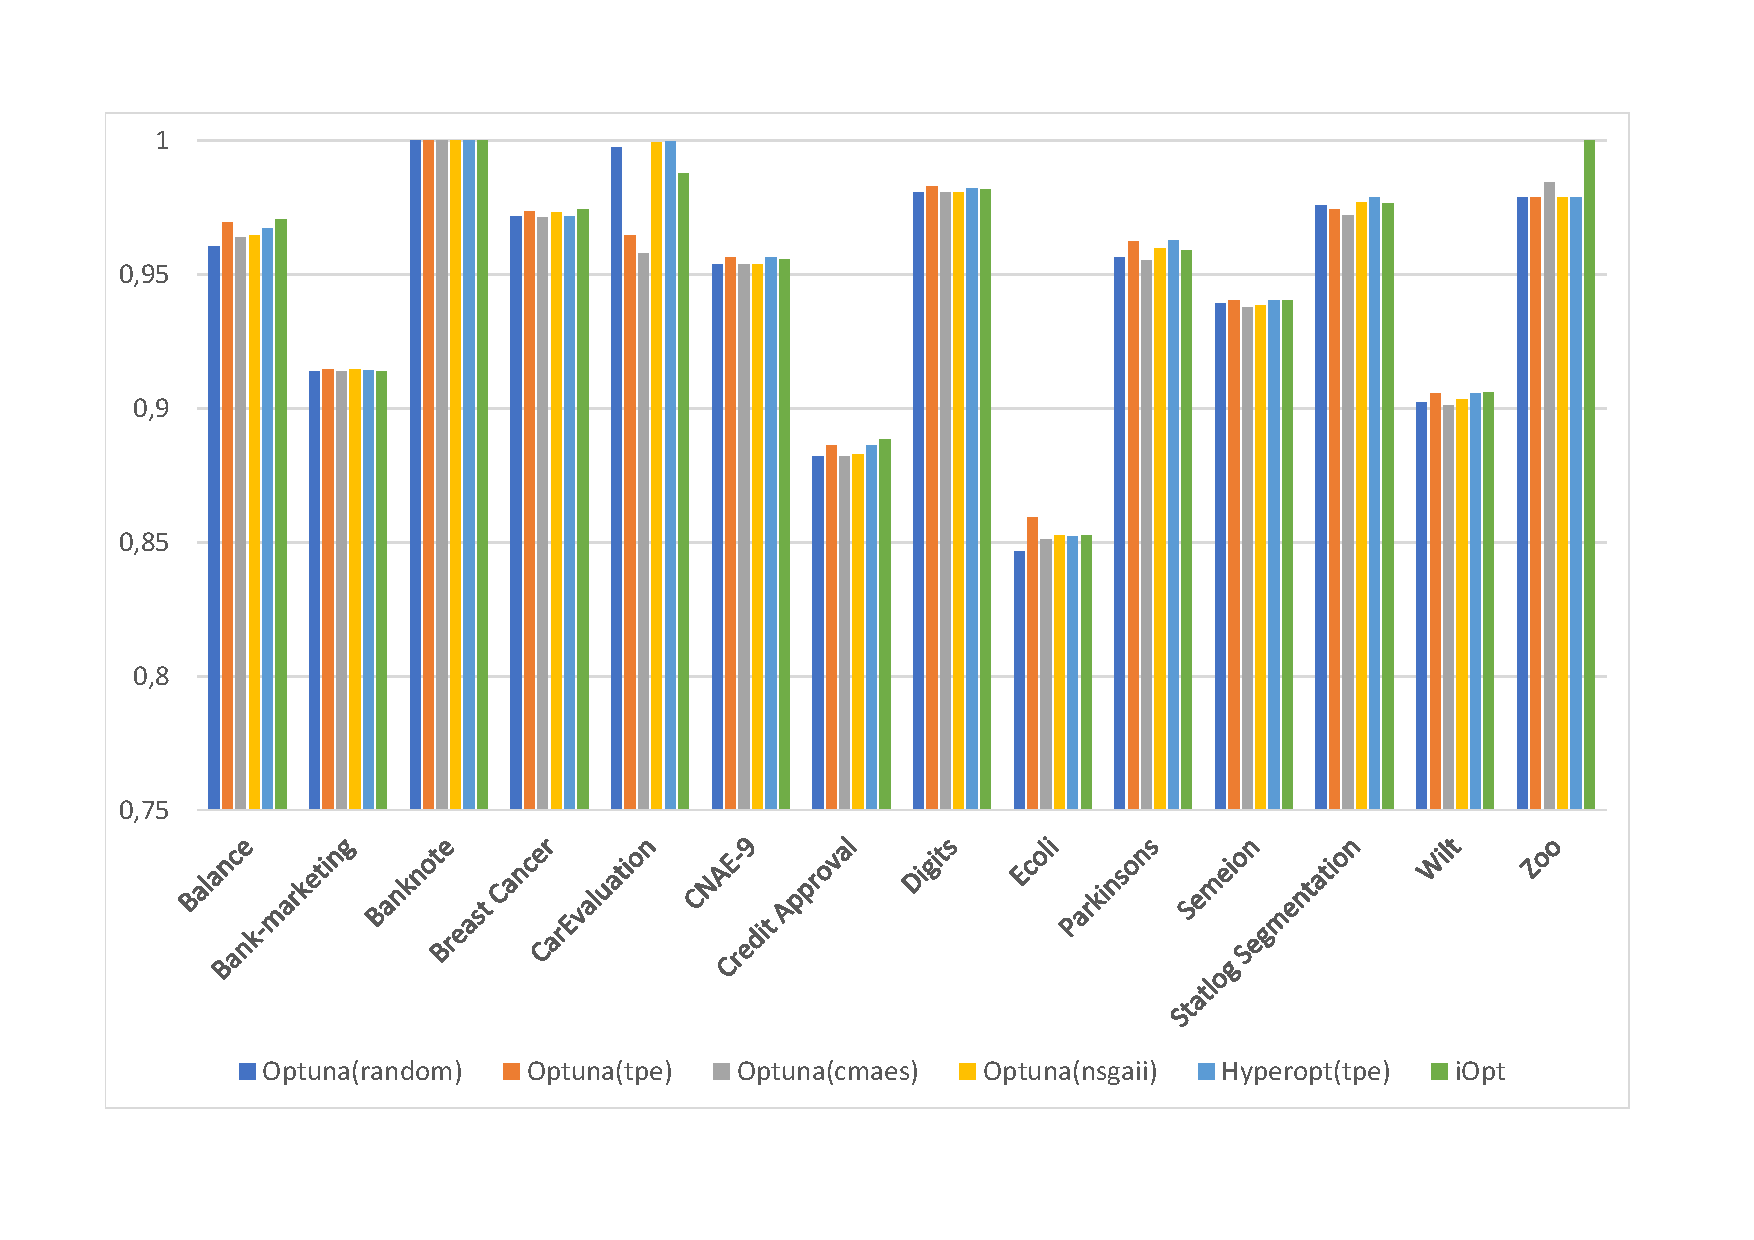
\includegraphics[width=0.85\textwidth]{MLP_1.pdf}
\caption{Values of the optimized metrics for the XGBoost algorithm, obtained in the worst case} \label{fig_res_5}
\end{figure}

\begin{figure}
\centering
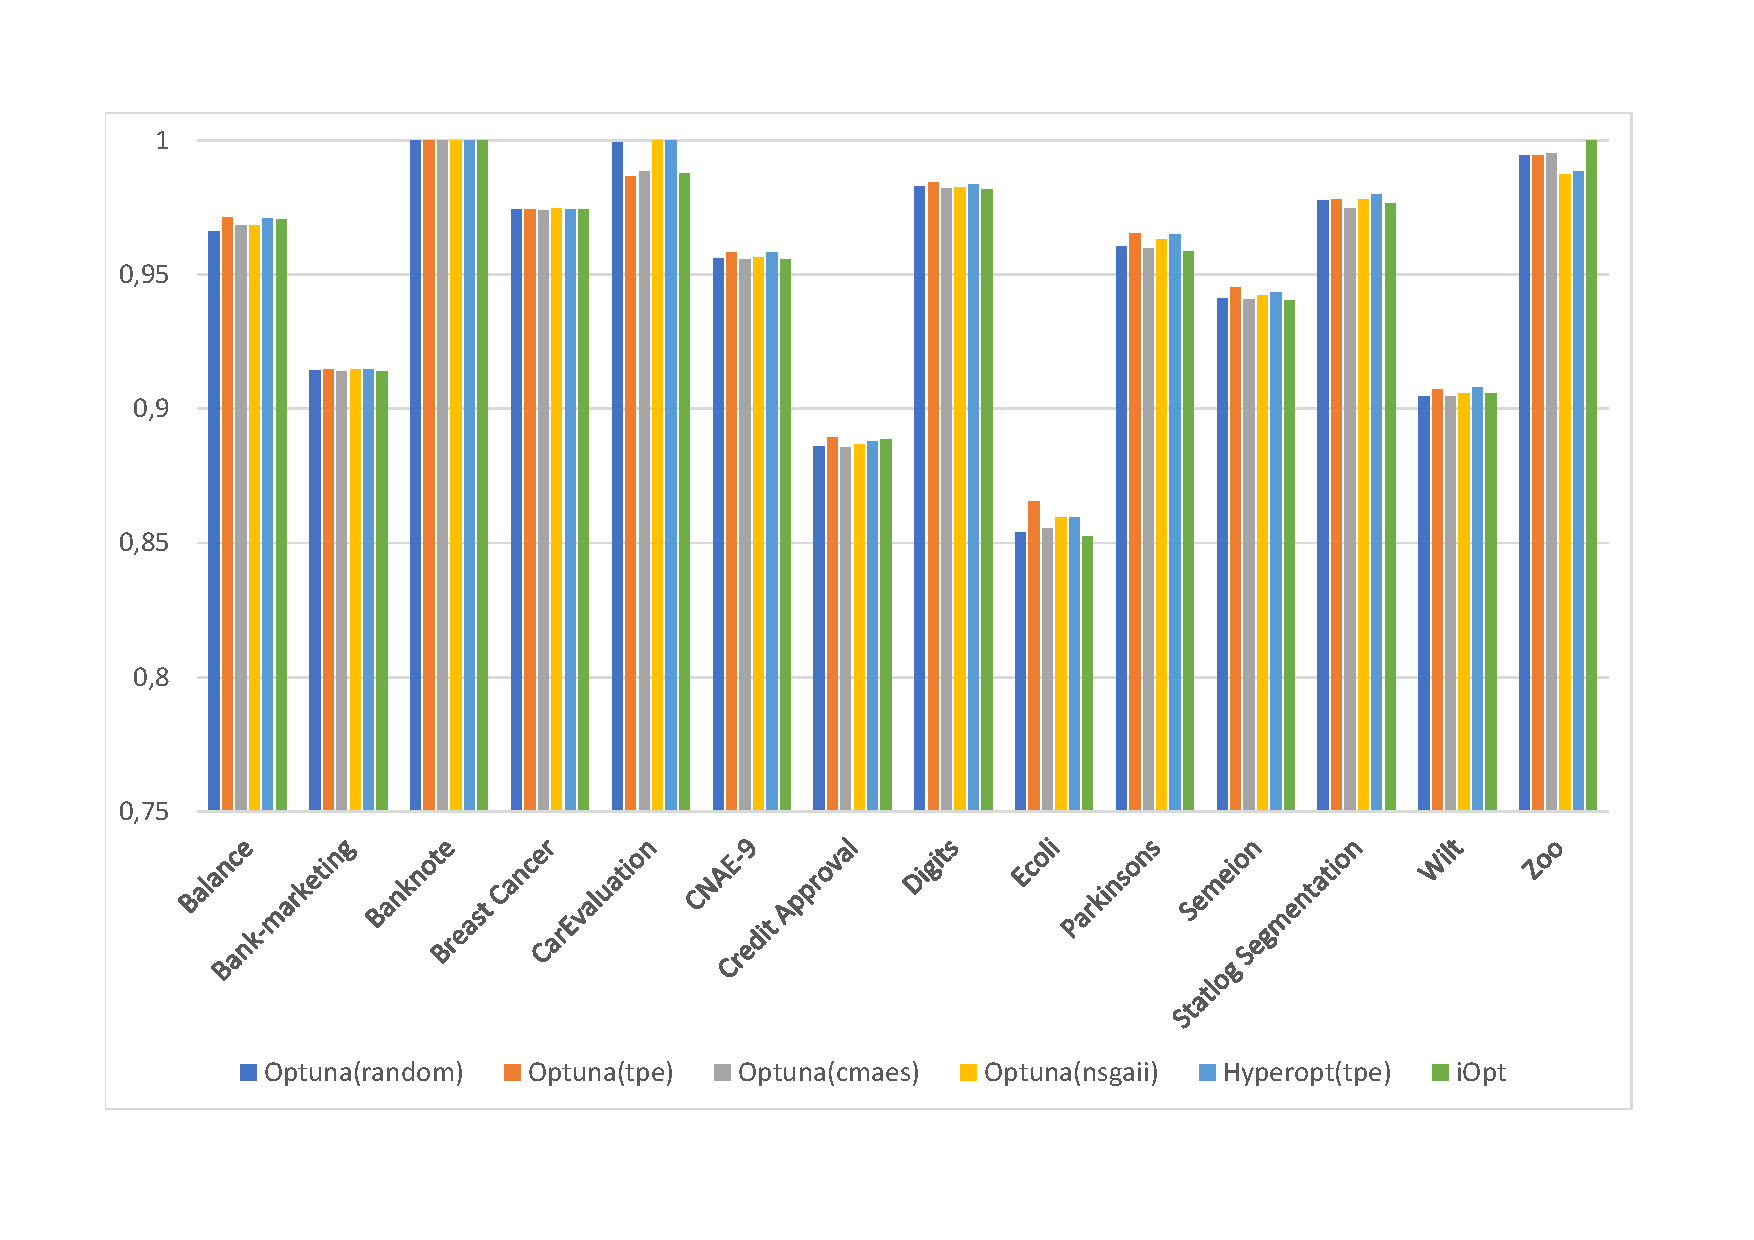
\includegraphics[width=0.85\textwidth]{MLP_2_avg.pdf}
\caption{Values of optimized metrics for the XGBoost algorithm averaged over 10 runs} \label{fig_res_6}
\end{figure}

Figures \ref{fig_res_5} and \ref{fig_res_6} show the values of classification metrics of the MLP algorithm. The iOpt framework performed better on the Balance, Bank-marketing, Banknote, Breast Cancer, Credit Approval, Wilt, Zoo datasets. Considering the average values of metrics on 10 runs of hyperparameter optimization, the Optuna framework performed better on the Breast Cancer, CNAE-9, Credit Approval, Digits, Ecoli, Parkinsons, Semeion datasets, and the Hyperopt on the Statlog Segmentation, Wilt, CarEvaluation datasets.


Thus, we can conclude that the iOpt framework shows comparable results with the Optuna and Hyperopt frameworks in terms of performance quality. It should be reminded that the algorithms implemented within the iOpt framework are deterministic. As a consequence, iOpt, unlike Optuna and Hyperopt, only needs to be run once to achieve the best values of the quality metric.

Next, we consider the performance of the iOpt, Optuna, and Hyperopt frameworks. Table \ref{tab:time} shows the running time of the frameworks for optimizing the hyperparameters.  A single optimization run was performed with a maximum number of 200 search trials. It is obvious that even in the case of a single run iOpt shows better performance on many datasets compared to Optuna and Hyperopt.

To obtain a good solution, the randomized methods from Optuna and Hyperopt should be repeated several times. In this case, the performance gain of iOpt is even greater. As an example, Figure \ref{fig8} shows a comparison of the runtime of the frameworks with 10 reruns of Optuna and Hyperopt on the Wilt dataset.


% Please add the following required packages to your document preamble:
% \usepackage{graphicx}
% \usepackage[table,xcdraw]{xcolor}
% If you use beamer only pass "xcolor=table" option, i.e. \documentclass[xcolor=table]{beamer}
\begin{table}[]
\centering
\caption{Values of optimized metrics for the algorithm's averaged over 10 runs}
\label{tab:res}
\resizebox{\textwidth}{!}{%
\begin{tabular}{ccccccc}
\hline
\textbf{Dataset}                & \textbf{iOpt}                         & \textbf{Optuna(random)}                        & \textbf{Optuna(tpe)}                           & \textbf{Optuna(cmaes)}                         & \textbf{Optuna(nsgaii)}                        & \textbf{Hyperopt(tpe)}                         \\ \hline
                                & \multicolumn{6}{c}{\textbf{SVM}}                                                                                                                                                                                                                                                           \\ \hline
\textbf{Balance}                & {\color[HTML]{FE0000} 0.856}          & 0.856 $\pm$ 0.07\%                                 & 0.856 $\pm$ 0.23\%                                 & 0.834 $\pm$ 8.81\%                                 & \textbf{0.857 $\pm$ 0.31\%}                        & 0.856 $\pm$ 0.07\%                                 \\
\textbf{Bank-marketing}         & {\color[HTML]{FE0000} 0.894}          & 0.880 $\pm$ 1.65\%                                 & 0.892 $\pm$ 2.11\%                                 & 0.861 $\pm$ 5.16\%                                 & 0.879 $\pm$ 3.45\%                                 & \textbf{0.896 $\pm$ 0.48\%}                        \\
\textbf{Banknote}               & {\color[HTML]{FE0000} \textbf{0.992}} & 0.990 $\pm$ 0.04\%                                 & 0.991 $\pm$ 0.07\%                                 & 0.990 $\pm$ 0.20\%                                 & 0.990 $\pm$ 0.02\%                                 & 0.990 $\pm$ 0.00\%                                 \\
\textbf{Breast Cancer}          & {\color[HTML]{FE0000} 0.971}          & 0.970 $\pm$ 0.13\%                                 & 0.972 $\pm$ 0.19\%                                 & \textbf{0.973 $\pm$ 0.25\%}                        & 0.972 $\pm$ 0.13\%                                 & \textbf{0.973 $\pm$ 0.26\%}                        \\
\textbf{CarEvaluation}          & 0.349                                 & 0.350 $\pm$ 4.83\%                                 & {\color[HTML]{FE0000} \textbf{0.376 $\pm$ 4.57\%}} & 0.349 $\pm$ 4.83\%                                 & 0.355 $\pm$ 3.77\%                                 & 0.366 $\pm$ 3.21\%                                 \\
\textbf{CNAE-9}                 & {\color[HTML]{FE0000} \textbf{0.941}} & 0.938 $\pm$ 0.07\%                                 & 0.939 $\pm$ 0.05\%                                 & 0.939 $\pm$ 0.00\%                                 & 0.938 $\pm$ 0.05\%                                 & 0.939 $\pm$ 0.07\%                                 \\
\textbf{Credit   Approval}      & 0.878                                 & 0.881 $\pm$ 0.22\%                                 & {\color[HTML]{FE0000} \textbf{0.884 $\pm$ 0.18\%}} & 0.880 $\pm$ 0.23\%                                 & 0.880 $\pm$ 0.22\%                                 & 0.881 $\pm$ 0.21\%                                 \\
\textbf{Digits}                 & 0.984                                 & 0.984 $\pm$ 0.06\%                                 & {\color[HTML]{FE0000} \textbf{0.985 $\pm$ 0.02\%}} & \textbf{0.985 $\pm$ 0.05\%}                        & 0.984 $\pm$ 0.06\%                                 & \textbf{0.985 $\pm$ 0.03\%}                        \\
\textbf{Ecoli}                  & {\color[HTML]{FE0000} \textbf{0.863}} & 0.855 $\pm$ 0.28\%                                 & 0.861 $\pm$ 0.45\%                                 & 0.860 $\pm$ 0.59\%                                 & 0.855 $\pm$ 0.15\%                                 & 0.859 $\pm$ 0.28\%                                 \\
\textbf{Parkinsons}             & {\color[HTML]{FE0000} \textbf{0.931}} & 0.929 $\pm$ 0.33\%                                 & 0.930 $\pm$ 0.28\%                                 & 0.930 $\pm$ 0.19\%                                 & \textbf{0.931 $\pm$ 0.39\%}                        & \textbf{0.931 $\pm$ 0.36\%}                        \\
\textbf{Semeion}                & {\color[HTML]{FE0000} \textbf{0.942}} & 0.941 $\pm$ 0.10\%                                 & 0.941 $\pm$ 0.19\%                                 & \textbf{0.942 $\pm$ 0.12\%}                        & 0.941 $\pm$ 0.10\%                                 & \textbf{0.942 $\pm$ 0.09\%}                        \\
\textbf{Statlog   Segmentation} & {\color[HTML]{FE0000} \textbf{0.958}} & 0.955 $\pm$ 0.13\%                                 & 0.957 $\pm$ 0.07\%                                 & 0.956 $\pm$ 0.08\%                                 & 0.956 $\pm$ 0.06\%                                 & 0.956 $\pm$ 0.06\%                                 \\
\textbf{Wilt}                   & {\color[HTML]{FE0000} \textbf{0.704}} & 0.681 $\pm$ 1.90\%                                 & 0.699 $\pm$ 1.95\%                                 & 0.659 $\pm$ 17.91\%                                & 0.674 $\pm$ 1.89\%                                 & 0.696 $\pm$ 1.07\%                                 \\
\textbf{Zoo}                    & {\color[HTML]{FE0000} \textbf{0.979}} & {\color[HTML]{FE0000} \textbf{0.979 $\pm$ 0.00\%}} & {\color[HTML]{FE0000} \textbf{0.979 $\pm$ 0.00\%}} & {\color[HTML]{FE0000} \textbf{0.979 $\pm$ 0.00\%}} & {\color[HTML]{FE0000} \textbf{0.979 $\pm$ 0.00\%}} & {\color[HTML]{FE0000} \textbf{0.979 $\pm$ 0.00\%}} \\ \hline
\textbf{}                       & \multicolumn{6}{c}{\textbf{XGBoost}}                                                                                                                                                                                                                                                       \\ \hline
\textbf{Balance}                & 0.633                                 & 0.638 $\pm$ 1.16\%                                 & 0.650 $\pm$ 3.26\%                                 & 0.650 $\pm$ 1.73\%                                 & 0.645 $\pm$ 1.50\%                                 & {\color[HTML]{FE0000} \textbf{0.661 $\pm$ 2.63\%}} \\
\textbf{Bank-marketing}         & 0.918                                 & 0.918 $\pm$ 0.04\%                                 & {\color[HTML]{FE0000} \textbf{0.919 $\pm$ 0.04\%}} & 0.918 $\pm$ 0.04\%                                 & 0.918 $\pm$ 0.03\%                                 & 0.918 $\pm$ 0.03\%                                 \\
\textbf{Banknote}               & 0.994                                 & 0.994 $\pm$ 0.07\%                                 & \textbf{0.996 $\pm$ 0.07\%}                        & {\color[HTML]{FE0000} \textbf{0.996 $\pm$ 0.08\%}} & 0.995 $\pm$ 0.08\%                                 & 0.995 $\pm$ 0.09\%                                 \\
\textbf{Breast Cancer}          & 0.961                                 & 0.957 $\pm$ 0.27\%                                 & {\color[HTML]{FE0000} \textbf{0.963 $\pm$ 0.16\%}} & 0.961 $\pm$ 0.17\%                                 & 0.960 $\pm$ 0.39\%                                 & 0.960 $\pm$ 0.25\%                                 \\
\textbf{CarEvaluation}          & {\color[HTML]{FE0000} 0.980}          & 0.965 $\pm$ 0.88\%                                 & \textbf{0.983 $\pm$ 0.39\%}                        & 0.980 $\pm$ 0.28\%                                 & 0.974 $\pm$ 0.48\%                                 & 0.977 $\pm$ 0.38\%                                 \\
\textbf{CNAE-9}                 & 0.932                                 & 0.924 $\pm$ 0.83\%                                 & {\color[HTML]{FE0000} \textbf{0.937 $\pm$ 0.34\%}} & 0.935 $\pm$ 0.26\%                                 & 0.930 $\pm$ 0.53\%                                 & 0.935 $\pm$ 0.29\%                                 \\
\textbf{Credit   Approval}      & {\color[HTML]{FE0000} \textbf{0.901}} & 0.897 $\pm$ 0.29\%                                 & \textbf{0.901 $\pm$ 0.30\%}                        & 0.898 $\pm$ 0.22\%                                 & 0.899 $\pm$ 0.32\%                                 & 0.898 $\pm$ 0.28\%                                 \\
\textbf{Digits}                 & 0.975                                 & 0.973 $\pm$ 0.17\%                                 & 0.976 $\pm$ 0.15\%                                 & {\color[HTML]{FE0000} \textbf{0.978 $\pm$ 0.15\%}} & 0.975 $\pm$ 0.15\%                                 & 0.976 $\pm$ 0.15\%                                 \\
\textbf{Ecoli}                  & {\color[HTML]{FE0000} \textbf{0.865}} & 0.852 $\pm$ 0.55\%                                 & \textbf{0.865 $\pm$ 0.53\%}                        & 0.864 $\pm$ 0.24\%                                 & 0.856 $\pm$ 0.40\%                                 & 0.861 $\pm$ 0.37\%                                 \\
\textbf{Parkinsons}             & {\color[HTML]{FE0000} 0.950}          & 0.944 $\pm$ 0.24\%                                 & \textbf{0.953 $\pm$ 0.42\%}                        & 0.952 $\pm$ 0.16\%                                 & 0.949 $\pm$ 0.32\%                                 & \textbf{0.953 $\pm$ 0.42\%}                        \\
\textbf{Semeion}                & 0.940                                 & 0.939 $\pm$ 0.48\%                                 & {\color[HTML]{FE0000} \textbf{0.951 $\pm$ 0.20\%}} & 0.950 $\pm$ 0.14\%                                 & 0.942 $\pm$ 0.39\%                                 & 0.948 $\pm$ 0.25\%                                 \\
\textbf{Statlog   Segmentation} & 0.982                                 & 0.981 $\pm$ 0.11\%                                 & \textbf{0.984 $\pm$ 0.24\%}                        & 0.984 $\pm$ 0.07\%                                 & 0.983 $\pm$ 0.13\%                                 & {\color[HTML]{FE0000} \textbf{0.984 $\pm$ 0.08\%}} \\
\textbf{Wilt}                   & 0.868                                 & 0.842 $\pm$ 1.41\%                                 & {\color[HTML]{FE0000} \textbf{0.872 $\pm$ 0.32\%}} & 0.867 $\pm$ 0.43\%                                 & 0.858 $\pm$ 0.88\%                                 & 0.865 $\pm$ 0.34\%                                 \\
\textbf{Zoo}                    & {\color[HTML]{FE0000} \textbf{1.000}} & 0.992 $\pm$ 0.86\%                                 & 0.992 $\pm$ 0.79\%                                 & 0.989 $\pm$ 0.73\%                                 & 0.998 $\pm$ 0.47\%                                 & 0.987 $\pm$ 0.64\%                                 \\ \hline
\textbf{}                       & \multicolumn{6}{c}{\textbf{MLP}}                                                                                                                                                                                                                                                           \\ \hline
\textbf{Balance}                & 0.968                                 & 0.967 $\pm$ 0.41\%                                 & {\color[HTML]{FE0000} \textbf{0.973 $\pm$ 0.30\%}} & 0.966 $\pm$ 0.39\%                                 & 0.969 $\pm$ 0.32\%                                 & 0.970 $\pm$ 0.32\%                                 \\
\textbf{Bank-marketing}         & 0.914                                 & 0.914 $\pm$ 0.05\%                                 & \textbf{0.915 $\pm$ 0.04\%}                        & 0.914 $\pm$ 0.03\%                                 & {\color[HTML]{FE0000} \textbf{0.915 $\pm$ 0.03\%}} & {\color[HTML]{FE0000} \textbf{0.915 $\pm$ 0.03\%}} \\
\textbf{Banknote}               & {\color[HTML]{FE0000} \textbf{1.000}} & {\color[HTML]{FE0000} \textbf{1.000 $\pm$ 0.00\%}} & {\color[HTML]{FE0000} \textbf{1.000 $\pm$ 0.00\%}} & {\color[HTML]{FE0000} \textbf{1.000 $\pm$ 0.00\%}} & {\color[HTML]{FE0000} \textbf{1.000 $\pm$ 0.00\%}} & {\color[HTML]{FE0000} \textbf{1.000 $\pm$ 0.00\%}} \\
\textbf{Breast Cancer}          & {\color[HTML]{FE0000} \textbf{0.974}} & \textbf{0.974 $\pm$ 0.16\%}                        & \textbf{0.974 $\pm$ 0.07\%}                        & 0.973 $\pm$ 0.12\%                                 & \textbf{0.974 $\pm$ 0.09\%}                        & \textbf{0.974 $\pm$ 0.11\%}                        \\
\textbf{CarEvaluation}          & 0.996                                 & 0.999 $\pm$ 0.10\%                                 & 0.993 $\pm$ 1.33\%                                 & 0.982 $\pm$ 1.98\%                                 & \textbf{1.000 $\pm$ 0.03\%}                        & {\color[HTML]{FE0000} \textbf{1.000 $\pm$ 0.00\%}} \\
\textbf{CNAE-9}                 & 0.957                                 & 0.955 $\pm$ 0.12\%                                 & 0.958 $\pm$ 0.06\%                                 & 0.955 $\pm$ 0.14\%                                 & 0.957 $\pm$ 0.15\%                                 & {\color[HTML]{FE0000} \textbf{0.959 $\pm$ 0.17\%}} \\
\textbf{Credit   Approval}      & 0.885                                 & 0.885 $\pm$ 0.19\%                                 & {\color[HTML]{FE0000} \textbf{0.889 $\pm$ 0.15\%}} & 0.885 $\pm$ 0.17\%                                 & 0.886 $\pm$ 0.20\%                                 & 0.888 $\pm$ 0.13\%                                 \\
\textbf{Digits}                 & {\color[HTML]{FE0000} \textbf{0.984}} & 0.983 $\pm$ 0.14\%                                 & \textbf{0.984 $\pm$ 0.06\%}                        & 0.982 $\pm$ 0.06\%                                 & 0.983 $\pm$ 0.09\%                                 & \textbf{0.984 $\pm$ 0.07\%}                        \\
\textbf{Ecoli}                  & 0.848                                 & 0.857 $\pm$ 0.42\%                                 & \textbf{0.861 $\pm$ 0.53\%}                        & 0.859 $\pm$ 0.40\%                                 & 0.857 $\pm$ 0.53\%                                 & {\color[HTML]{FE0000} \textbf{0.861 $\pm$ 0.41\%}} \\
\textbf{Parkinsons}             & {\color[HTML]{FE0000} 0.963}          & 0.961 $\pm$ 0.28\%                                 & 0.965 $\pm$ 0.27\%                                 & 0.959 $\pm$ 0.32\%                                 & 0.962 $\pm$ 0.20\%                                 & \textbf{0.964 $\pm$ 0.30\%}                        \\
\textbf{Semeion}                & {\color[HTML]{FE0000} 0.945}          & 0.941 $\pm$ 0.14\%                                 & \textbf{0.946 $\pm$ 0.23\%}                        & 0.940 $\pm$ 0.11\%                                 & 0.943 $\pm$ 0.28\%                                 & 0.945 $\pm$ 0.15\%                                 \\
\textbf{Statlog   Segmentation} & 0.976                                 & 0.977 $\pm$ 0.12\%                                 & \textbf{0.979 $\pm$ 0.17\%}                        & 0.976 $\pm$ 0.18\%                                 & 0.978 $\pm$ 0.04\%                                 & {\color[HTML]{FE0000} \textbf{0.979 $\pm$ 0.04\%}} \\
\textbf{Wilt}                   & {\color[HTML]{FE0000} 0.906}          & 0.904 $\pm$ 0.15\%                                 & \textbf{0.907 $\pm$ 0.26\%}                        & 0.906 $\pm$ 0.23\%                                 & 0.906 $\pm$ 0.03\%                                 & \textbf{0.907 $\pm$ 0.14\%}                        \\
\textbf{Zoo}                    & {\color[HTML]{FE0000} \textbf{1.000}} & 0.988 $\pm$ 0.97\%                                 & 0.990 $\pm$ 0.90\%                                 & 0.995 $\pm$ 0.80\%                                 & 0.996 $\pm$ 0.86\%                                 & 0.995 $\pm$ 0.81\%                                 \\ \hline
\end{tabular}%
}
\end{table}

% Please add the following required packages to your document preamble:
% \usepackage{graphicx}
\begin{table}[]
\centering
\caption{Time of hyperparameter tuning.}
\label{tab:time}
\resizebox{\textwidth}{!}{%
\begin{tabular}{cccccc}
\hline
\textbf{Dataset}                & \textbf{iOpt}     & \textbf{Optuna(tpe)}        & \textbf{Optuna(cmaes)} & \textbf{Optuna(nsgaii)}    & \textbf{Hyperopt(tpe)}      \\ \hline
                                & \multicolumn{5}{c}{\textbf{SVM}}                                                                                                    \\ \hline
\textbf{Balance}                & \textbf{00:00:15} & 00:00:19 ± 0.66\%           & 00:00:17 ± 8.71\%      & 00:00:20 ± 3.00\%          & 00:00:21 ± 4.44\%           \\
\textbf{Bank-marketing}         & \textbf{01:31:18} & 02:02:05 ± 4.12\%           & 01:49:42 ± 8.35\%      & 01:51:06 ± 4.62\%          & 01:52:03 ± 8.25\%           \\
\textbf{Banknote}               & 00:00:35          & \textbf{00:00:25 ± 3.60\%}  & 00:00:32 ± 10.86\%     & 00:00:48 ± 5.89\%          & 00:00:39 ± 4.37\%           \\
\textbf{Breast Cancer}          & \textbf{00:00:11} & 00:00:15 ± 1.38\%           & 00:00:14 ± 3.45\%      & 00:00:16 ± 4.59\%          & 00:00:18 ± 3.79\%           \\
\textbf{CarEvaluation}          & \textbf{00:01:21} & 00:01:48 ± 2.82\%           & 00:01:28 ± 6.69\%      & 00:01:34 ± 2.01\%          & 00:01:44 ± 3.10\%           \\
\textbf{CNAE-9}                 & \textbf{00:05:53} & 00:08:24 ± 18.64\%          & 00:08:30 ± 3.92\%      & 00:08:27 ± 2.28\%          & 00:08:22 ± 5.14\%           \\
\textbf{Credit   Approval}      & \textbf{00:00:19} & 00:00:26 ± 16.46\%          & 00:00:21 ± 7.39\%      & 00:00:23 ± 2.38\%          & 00:00:25 ± 4.47\%           \\
\textbf{Digits}                 & 00:02:07          & \textbf{00:02:01 ± 5.04\%}  & 00:02:47 ± 7.83\%      & 00:03:35 ± 7.10\%          & 00:03:09 ± 4.74\%           \\
\textbf{Ecoli}                  & \textbf{00:00:08} & 00:00:13 ± 2.09\%           & 00:00:10 ± 2.28\%      & 00:00:10 ± 1.66\%          & 00:00:14 ± 3.30\%           \\
\textbf{Parkinsons}             & \textbf{00:00:07} & 00:00:11 ± 1.38\%           & 00:00:08 ± 0.96\%      & 00:00:08 ± 1.43\%          & 00:00:12 ± 4.09\%           \\
\textbf{Semeion}                & \textbf{00:04:03} & 00:04:16 ± 5.22\%           & 00:05:17 ± 3.24\%      & 00:05:51 ± 1.73\%          & 00:05:57 ± 3.06\%           \\
\textbf{Statlog   Segmentation} & 00:02:07          & \textbf{00:01:45 ± 4.02\%}  & 00:02:59 ± 5.75\%      & 00:04:12 ± 6.43\%          & 00:03:05 ± 4.06\%           \\
\textbf{Wilt}                   & \textbf{00:01:51} & 00:02:17 ± 6.65\%           & 00:02:01 ± 9.83\%      & 00:02:07 ± 3.28\%          & 00:02:16 ± 4.78\%           \\
\textbf{Zoo}                    & \textbf{00:00:05} & 00:00:10 ± 2.08\%           & 00:00:07 ± 1.73\%      & 00:00:07 ± 2.42\%          & 00:00:10 ± 3.47\%           \\ \hline
                                & \multicolumn{5}{c}{\textbf{XGBoost}}                                                                                                \\ \hline
\textbf{Balance}                & \textbf{00:01:49} & 00:03:38 ± 10.57\%          & 00:03:09 ± 10.94\%     & 00:02:36 ± 6.39\%          & 00:02:55 ± 11.63\%          \\
\textbf{Bank-marketing}         & 01:46:27          & 01:52:51 ± 17.65\%          & 02:06:44 ± 14.76\%     & 01:51:28 ± 7.79\%          & \textbf{01:43:15 ± 13.30\%} \\
\textbf{Banknote}               & \textbf{00:02:02} & 00:03:36 ± 18.51\%          & 00:03:15 ± 10.33\%     & 00:02:35 ± 6.93\%          & 00:02:45 ± 5.20\%           \\
\textbf{Breast Cancer}          & \textbf{00:01:45} & 00:03:25 ± 26.50\%          & 00:02:33 ± 19.95\%     & 00:02:31 ± 13.55\%         & 00:02:26 ± 8.54\%           \\
\textbf{CarEvaluation}          & 00:10:10          & 00:12:05 ± 8.62\%           & 00:10:53 ± 8.07\%      & 00:07:14 ± 6.79\%          & \textbf{00:07:42 ± 12.51\%} \\
\textbf{CNAE-9}                 & 03:47:42          & 04:55:03 ± 26.76\%          & 05:43:27 ± 14.35\%     & 03:55:49 ± 13.82\%         & \textbf{03:42:39 ± 18.30\%} \\
\textbf{Credit   Approval}      & \textbf{00:01:30} & 00:02:27 ± 23.63\%          & 00:01:54 ± 23.08\%     & 00:01:58 ± 6.65\%          & 00:01:44 ± 13.34\%          \\
\textbf{Digits}                 & 00:48:57          & 00:59:09 ± 21.83\%          & 00:54:27 ± 8.20\%      & 00:43:35 ± 9.93\%          & \textbf{00:46:52 ± 8.24\%}  \\
\textbf{Ecoli}                  & \textbf{00:02:40} & 00:04:03 ± 21.05\%          & 00:03:30 ± 22.08\%     & 00:02:48 ± 8.63\%          & 00:03:05 ± 8.97\%           \\
\textbf{Parkinsons}             & \textbf{00:01:09} & 00:02:32 ± 16.25\%          & 00:01:52 ± 12.30\%     & 00:01:34 ± 4.24\%          & 00:01:45 ± 12.30\%          \\
\textbf{Semeion}                & 01:52:08          & 01:19:57 ± 12.21\%          & 01:42:52 ± 14.47\%     & 02:01:16 ± 9.22\%          & \textbf{01:41:40 ± 7.68\%}  \\
\textbf{Statlog   Segmentation} & 00:34:59          & 00:43:59 ± 13.68\%          & 00:38:13 ± 6.14\%      & \textbf{00:25:03 ± 8.20\%} & 00:32:15 ± 8.61\%           \\
\textbf{Wilt}                   & 00:06:44          & 00:10:42 ± 6.89\%           & 00:08:20 ± 7.94\%      & \textbf{00:06:11 ± 8.76\%} & 00:08:09 ± 8.43\%           \\
\textbf{Zoo}                    & \textbf{00:01:47} & 00:02:53 ± 20.08\%          & 00:02:21 ± 16.16\%     & 00:02:05 ± 4.28\%          & 00:02:13 ± 9.09\%           \\ \hline
                                & \multicolumn{5}{c}{\textbf{MLP}}                                                                                                    \\ \hline
\textbf{Balance}                & \textbf{00:09:29} & 00:18:14 ± 61.97\%          & 00:26:45 ± 11.25\%     & 00:20:55 ± 11.15\%         & 00:15:37 ± 10.06\%          \\
\textbf{Bank-marketing}         & 06:10:05          & \textbf{04:42:08 ± 39.48\%} & 05:44:30 ± 15.70\%     & 07:04:15 ± 10.63\%         & 08:11:02 ± 16.22\%          \\
\textbf{Banknote}               & \textbf{02:07:36} & 02:29:16 ± 44.57\%          & 04:43:15 ± 13.11\%     & 03:20:56 ± 8.58\%          & 02:39:20 ± 11.03\%          \\
\textbf{Breast Cancer}          & \textbf{00:43:14} & 02:48:26 ± 10.35\%          & 02:41:29 ± 15.72\%     & 02:46:45 ± 5.13\%          & 02:11:56 ± 29.01\%          \\
\textbf{CarEvaluation}          & \textbf{02:08:22} & 04:21:15 ± 17.08\%          & 03:04:09 ± 12.40\%     & 03:45:18 ± 9.32\%          & 03:55:44 ± 19.04\%          \\
\textbf{CNAE-9}                 & 07:46:15          & \textbf{07:26:02 ± 9.33\%}  & 13:29:53 ± 11.28\%     & 10:57:27 ± 12.39\%         & 08:32:12 ± 7.19\%           \\
\textbf{Credit   Approval}      & \textbf{00:43:32} & 02:41:30 ± 10.89\%          & 02:24:56 ± 15.16\%     & 02:39:29 ± 4.92\%          & 01:57:22 ± 29.27\%          \\
\textbf{Digits}                 & \textbf{02:58:50} & 10:50:47 ± 7.21\%           & 09:30:39 ± 5.32\%      & 10:19:20 ± 6.95\%          & 08:45:23 ± 29.04\%          \\
\textbf{Ecoli}                  & \textbf{00:05:52} & 00:08:21 ± 16.93\%          & 00:07:03 ± 16.70\%     & 00:08:08 ± 7.34\%          & 00:07:01 ± 12.44\%          \\
\textbf{Parkinsons}             & \textbf{00:16:21} & 00:46:32 ± 34.33\%          & 00:49:54 ± 14.73\%     & 00:44:24 ± 5.05\%          & 00:34:48 ± 14.89\%          \\
\textbf{Semeion}                & \textbf{03:38:23} & 11:26:28 ± 25.20\%          & 10:19:44 ± 7.97\%      & 09:01:10 ± 13.98\%         & 07:55:17 ± 20.55\%          \\
\textbf{Statlog   Segmentation} & \textbf{00:48:57} & 19:27:00 ± 15.47\%          & 17:09:16 ± 11.57\%     & 17:02:03 ± 3.17\%          & 11:20:02 ± 3.89\%           \\
\textbf{Wilt}                   & \textbf{01:23:04} & 17:57:58 ± 28.49\%          & 19:23:37 ± 11.57\%     & 22:06:21 ± 9.34\%          & 12:38:43 ± 3.14\%           \\
\textbf{Zoo}                    & 00:01:46          & 00:01:52 ± 22.83\%          & 00:01:58 ± 7.72\%      & \textbf{00:01:40 ± 8.30\%} & 00:02:01 ± 12.96\%          \\ \hline
\end{tabular}%
}
\end{table}

%\begin{table}[ht]
%\caption{Time of hyperparameter tuning for a single run of algorithms.}
%\label{tab:3}
%\begin{tabular}{lllllll}
%\hline
%Dataset &
%  \begin{tabular}[c]{@{}l@{}}Optuna \\ random\end{tabular} &
%  \begin{tabular}[c]{@{}l@{}}Optuna \\ tpe\end{tabular} &
%  \begin{tabular}[c]{@{}l@{}}Optuna \\ cmaes\end{tabular} &
%  \begin{tabular}[c]{@{}l@{}}Optuna \\ nsgaii\end{tabular} &
%  \begin{tabular}[c]{@{}l@{}}Hyperopt\\ tpe\end{tabular} &
%  iOpt \\ \hline
%Balance                                                         & 10.8   & 9.2    & 9.0    & 10.6   & 10.3   & \textbf{7.7}    \\
%\begin{tabular}[c]{@{}l@{}}Bank \\ Marketing\end{tabular}       & 2888.5 & 3406.5 & \textbf{2704.7} & 3078.6 & 3190.3 & 2963.3 \\
%Banknote                                                        & 31.9   & \textbf{12.0}   & 17.7   & 22.1   & 21.7   & 18.4   \\
%\begin{tabular}[c]{@{}l@{}}Breast \\ Cancer\end{tabular}        & 9.3    & 7.6    & 6.3    & 8.1    & 8.5    & \textbf{6.0}    \\
%CarEvaluation                                                   & 50.9   & 63.3   & 51.0   & 53.1   & 69.5   & \textbf{45.2}   \\
%CNAE9                                                           & 295.6  & 207.6  & 318.4  & 262.2  & 253.5  & \textbf{144.9}  \\
%\begin{tabular}[c]{@{}l@{}}Credit \\ Approval\end{tabular}      & 14.2   & 12.6   & 13.4   & 13.4   & 15.8   & \textbf{10.8}   \\
%Digits                                                          & 132.8  & \textbf{57.5}   & 82.1   & 111.6  & 92.4   & 62.5   \\
%Ecoli                                                           & 5.5    & 6.3    & 4.0    & 5.4    & 6.4    & \textbf{3.6}    \\
%Parkinsons                                                      & 3.5    & 5.0    & 3.6    & 3.8    & 4.4    & \textbf{2.9}    \\
%Semeion                                                         & 218.4  & 119.5  & 157.9  & 135.7  & 193.6  & \textbf{114.2}  \\
%\begin{tabular}[c]{@{}l@{}}Statlog \\ Segmentation\end{tabular} & 156.1  & \textbf{55.4}   & 87.1   & 159.2  & 91.6   & 66.5   \\
%Wilt                                                            & 70.0   & 75.8   & 68.5   & 67.4   & 78.2   & \textbf{60.9}   \\
%Zoo                                                             & 3.0    & 3.9    & 3.0    & 3.1    & 4.2    & \textbf{1.8}    \\ \hline
%\end{tabular}
%\end{table}


\begin{figure}
\centering
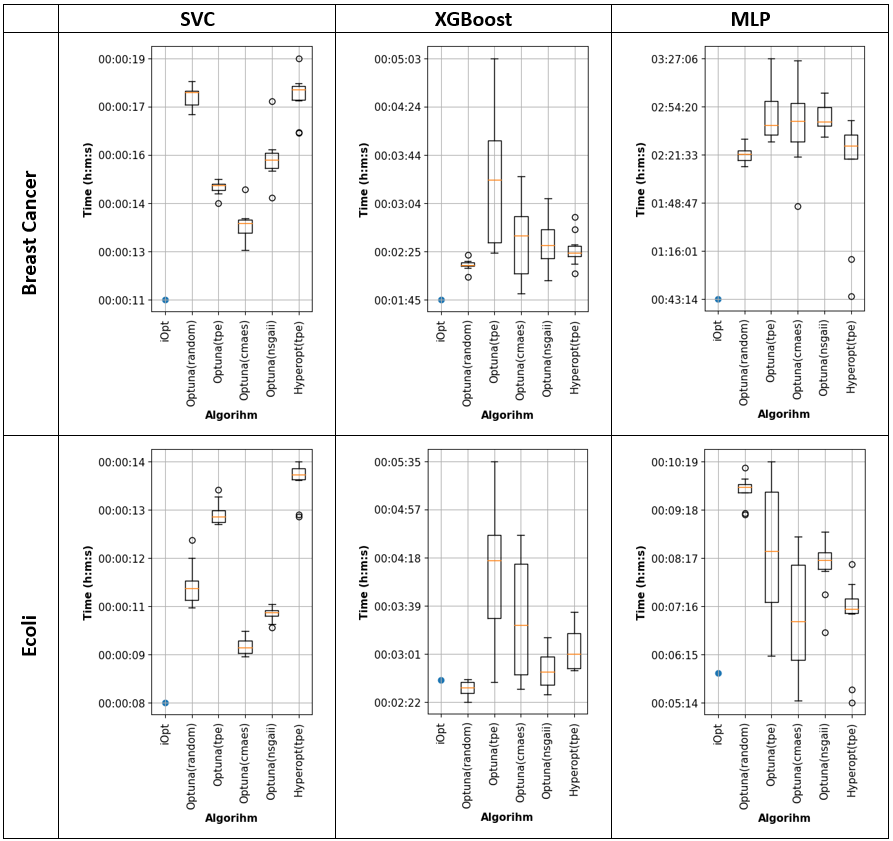
\includegraphics[width=\textwidth]{fig_time}
\caption{Time for tuning hyperparameters of the SVC algorithm to obtain good values of quality metrics on the Wilt dataset} \label{fig8}
\end{figure}

\section{Conclusion}
In this paper, we propose a hyperparameter tuning method that is based on the ideas of Lipschitz global optimization. In particular, we use a global search algorithm combined with dimensionality reduction based on Peano curves. We have proposed a generalization of Lipschitz optimization methods to the case of problems with partially integer variables, since many tunable algorithms have discrete hyperparameters.

We have tested our newly developed iOpt framework on real datasets, and experimental results show that our method can search for hyperparameters with comparable (and often better) values of the objective metric. At the same time, due to its deterministic nature, our method provides a stable result at any run, whereas known randomized algorithms need to be run several times to achieve a good result. This ensures a significant superiority of our framework in terms of the time required to select the optimal variant.

In the future, we plan to implement the parallelization of our algorithm, with a focus on heterogeneous computing systems. This will allow us to perform hyperparameter tuning of deep neural networks, which requires significant resources and cannot be performed in an acceptable time on a single computing device.


\section*{CRediT authorship contribution statement}

\textbf{Konstantin Barkalov:} Supervision, Conceptualization, Writing - original draft.
\textbf{Denis Karchkov:} Software, Data curation.
\textbf{Evgeny Kozinov:} Methodology, Validation, Writing - original draft.
\textbf{Ilya Lebedev:} Software, Investigation, Writing - original draft.
\textbf{Denis Rodionov:} Software, Investigation.
\textbf{Marina Usova:} Visualization.


\section*{Declaration of competing interest}

The authors declare that they have no known competing financial interests or personal relationships that could have appeared to influence the work reported in this paper.

\section*{Code availability}
The software that implements all of the described methods is available in the open repository \url{https://github.com/aimclub/iOpt/}.
Python scripts that reproduce the results of the experiments described in this paper are available at \url{https://github.com/aimclub/iOpt/benchmarks}.

\section*{Acknowledgements}
This work was supported by the Analytical Center for the Government of the Russian Federation (IGK 000000D730321P5Q0002), agreement No. 70-2021-00141.


%% The Appendices part is started with the command \appendix;
%% appendix sections are then done as normal sections
%% \appendix

%% \section{}
%% \label{}

%% If you have bibdatabase file and want bibtex to generate the
%% bibitems, please use
%%
\bibliographystyle{elsarticle-num} 
\bibliography{bibliography}

%% else use the following coding to input the bibitems directly in the
%% TeX file.

%\begin{thebibliography}{00}

%% \bibitem{label}
%% Text of bibliographic item

%\bibitem{}

%\end{thebibliography}
\end{document}
\endinput
%%
%% End of file `elsarticle-template-num.tex'.
